\section{Composites}

	\large{\bfseries{LGP}}
	\vspace{5mm}
	
		\normalsize
		{	
			The LGP (Linux group policy) name-space represents the top logical level of the software product.  It is also the name-space that encapsulates 
			to entry point for the application or executable.   
			\newline
			\newline
			The two primary classes in the following diagram namely LGPWindow and Splash.
			Splash is the window used to display the loading information to the user. This loading information is provided by the Framework and presented
			to the user to indicate which modules are being loaded.  
			\newline
			\newline
			Secondly the LGPWindow is the main window of the application to which UserControls (System.Controls.UserControl)
			(a derived class of System.Controls.Window in Windows Presentation Foundation) are shown.
		}
		
		\vspace{5mm}
	
		\begin{figurehere}
			\centering
			
\includegraphics[scale=0.4]{pages/appendix3/figures/dllscreens/lgp.png}
			\caption{LGP}
		\end{figurehere}
		
		
\newpage
	
	
	\large{\bfseries{LGP.Components.Factory}}
	\vspace{5mm}
	
		\begin{figurehere}
			\centering
			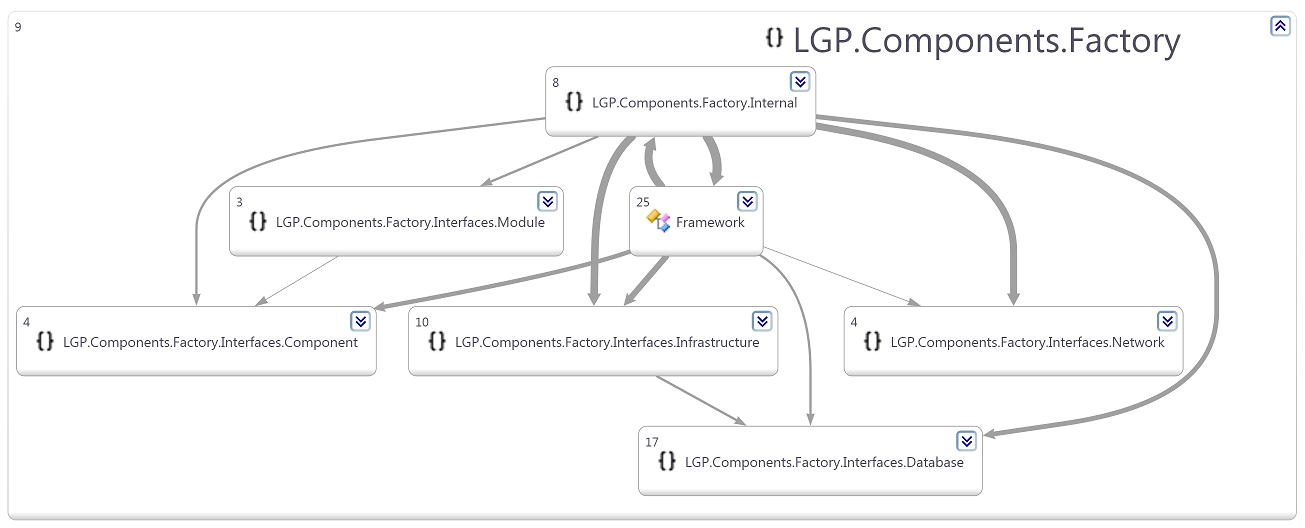
\includegraphics[scale=0.6,angle=90]{pages/appendix3/figures/dllscreens/factory.png}
		\caption{LGP.Components.Factory}
		\end{figurehere}
	
	\newpage
	
	
	\large{\bfseries{LGP.Components.Database}}
	\vspace{5mm}
	
		\begin{figurehere}
			\centering
			
\includegraphics[scale=0.8,angle=90]{pages/appendix3/figures/dllscreens/database.png}
			\caption{LGP.Components.Database}
		\end{figurehere}
	
	
\newpage
		
		
	\begin{multicols}{2}
	
		\large{\bfseries{LGP.Components.Database.Mysql}}
		\vspace{5mm}
		
			\begin{figurehere}
				\centering
				
\includegraphics[scale=0.35]{pages/appendix3/figures/dllscreens/mysql.png}
				\caption{LGP.Components.Database.Mysql}
			\end{figurehere}
					
		
		\large{\bfseries{LGP.Components.Database.Mssql}}
		\vspace{5mm}
		
			\begin{figurehere}
				\centering
				
\includegraphics[scale=0.35]{pages/appendix3/figures/dllscreens/mssql.png}
				\caption{LGP.Components.Database.Mssql}
			\end{figurehere}
		
		\columnbreak
		
				
		\large{\bfseries{LGP.Components.Database.Oracle}}
		\vspace{5mm}
		
			\begin{figurehere}
				\centering
				
\includegraphics[scale=0.35]{pages/appendix3/figures/dllscreens/oracle.png}
				\caption{LGP.Components.Database.Oracle}
			\end{figurehere}
		
		

		\large{\bfseries{LGP.Components.Database.Postgresql}}
		\vspace{5mm}
		
			\begin{figurehere}
				\centering
				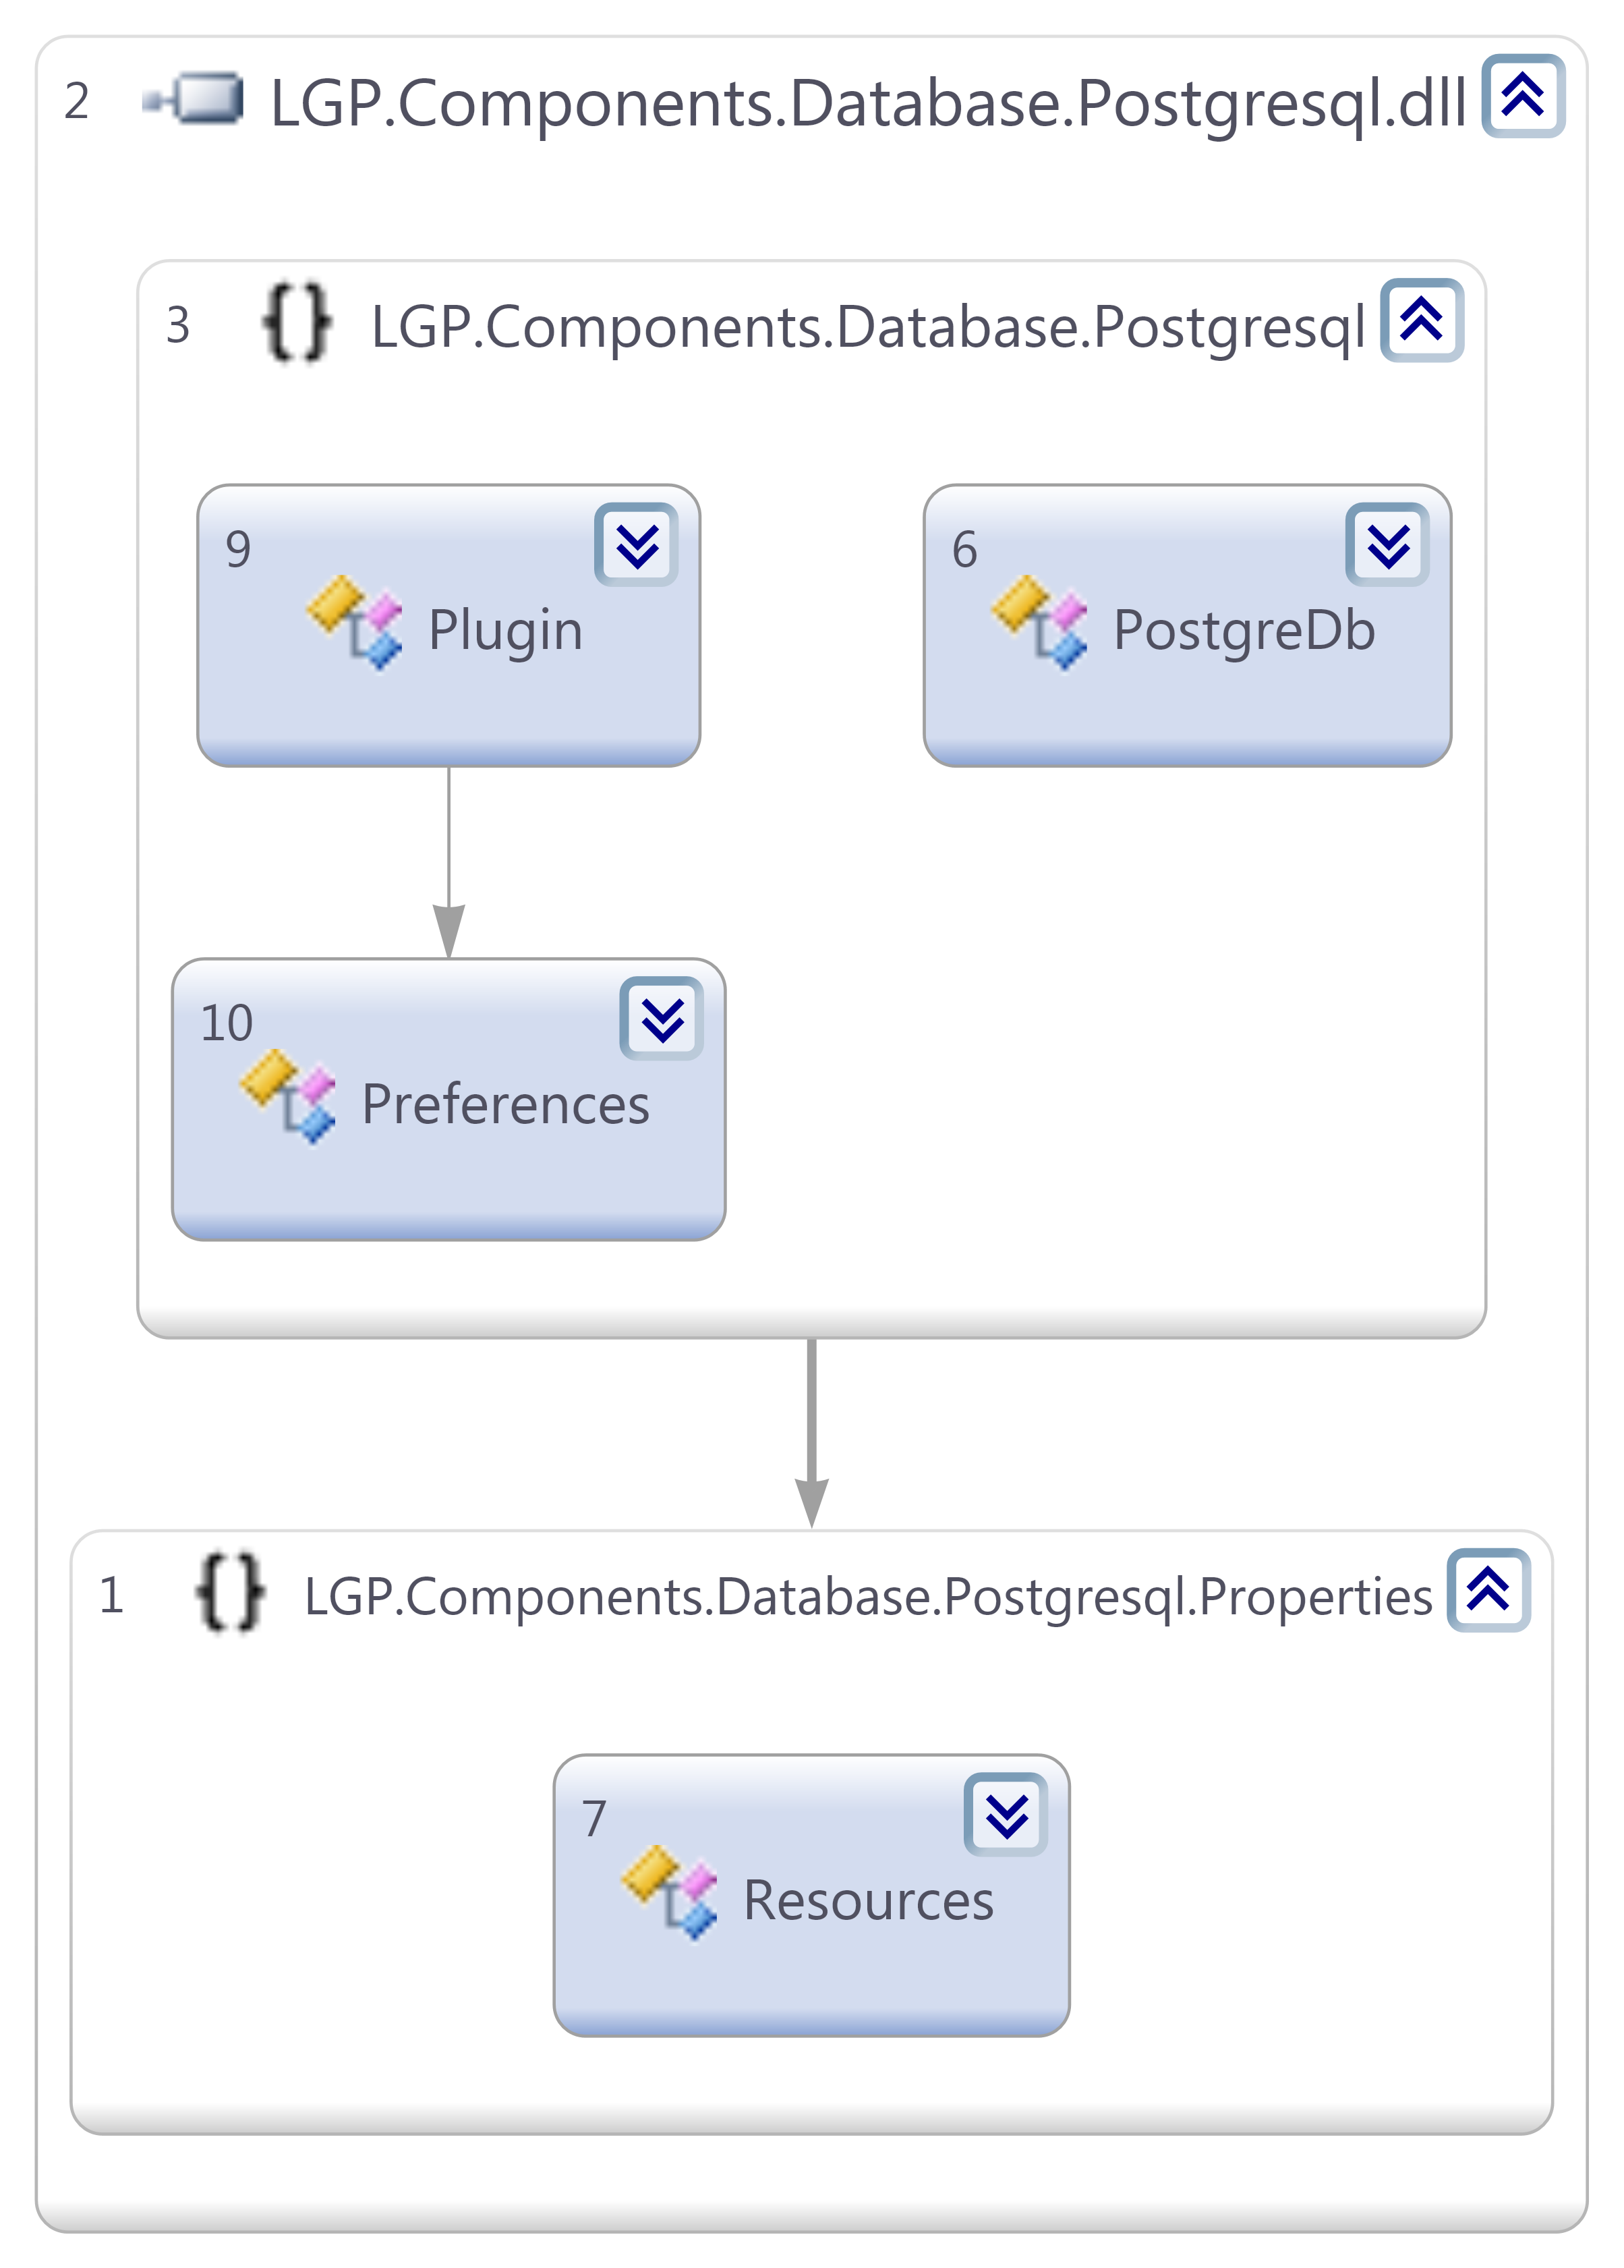
\includegraphics[scale=0.35]{pages/appendix3/figures/dllscreens/postgresql.png}
				\caption{LGP.Components.Database.Postgresql}
			\end{figurehere}
		
	\end{multicols}
	
			
\newpage	
	
			
	\begin{multicols}{2}	

		\large{\bfseries{LGP.Components.Notifications}}
		\vspace{5mm}
		
			\begin{figurehere}
				\centering
				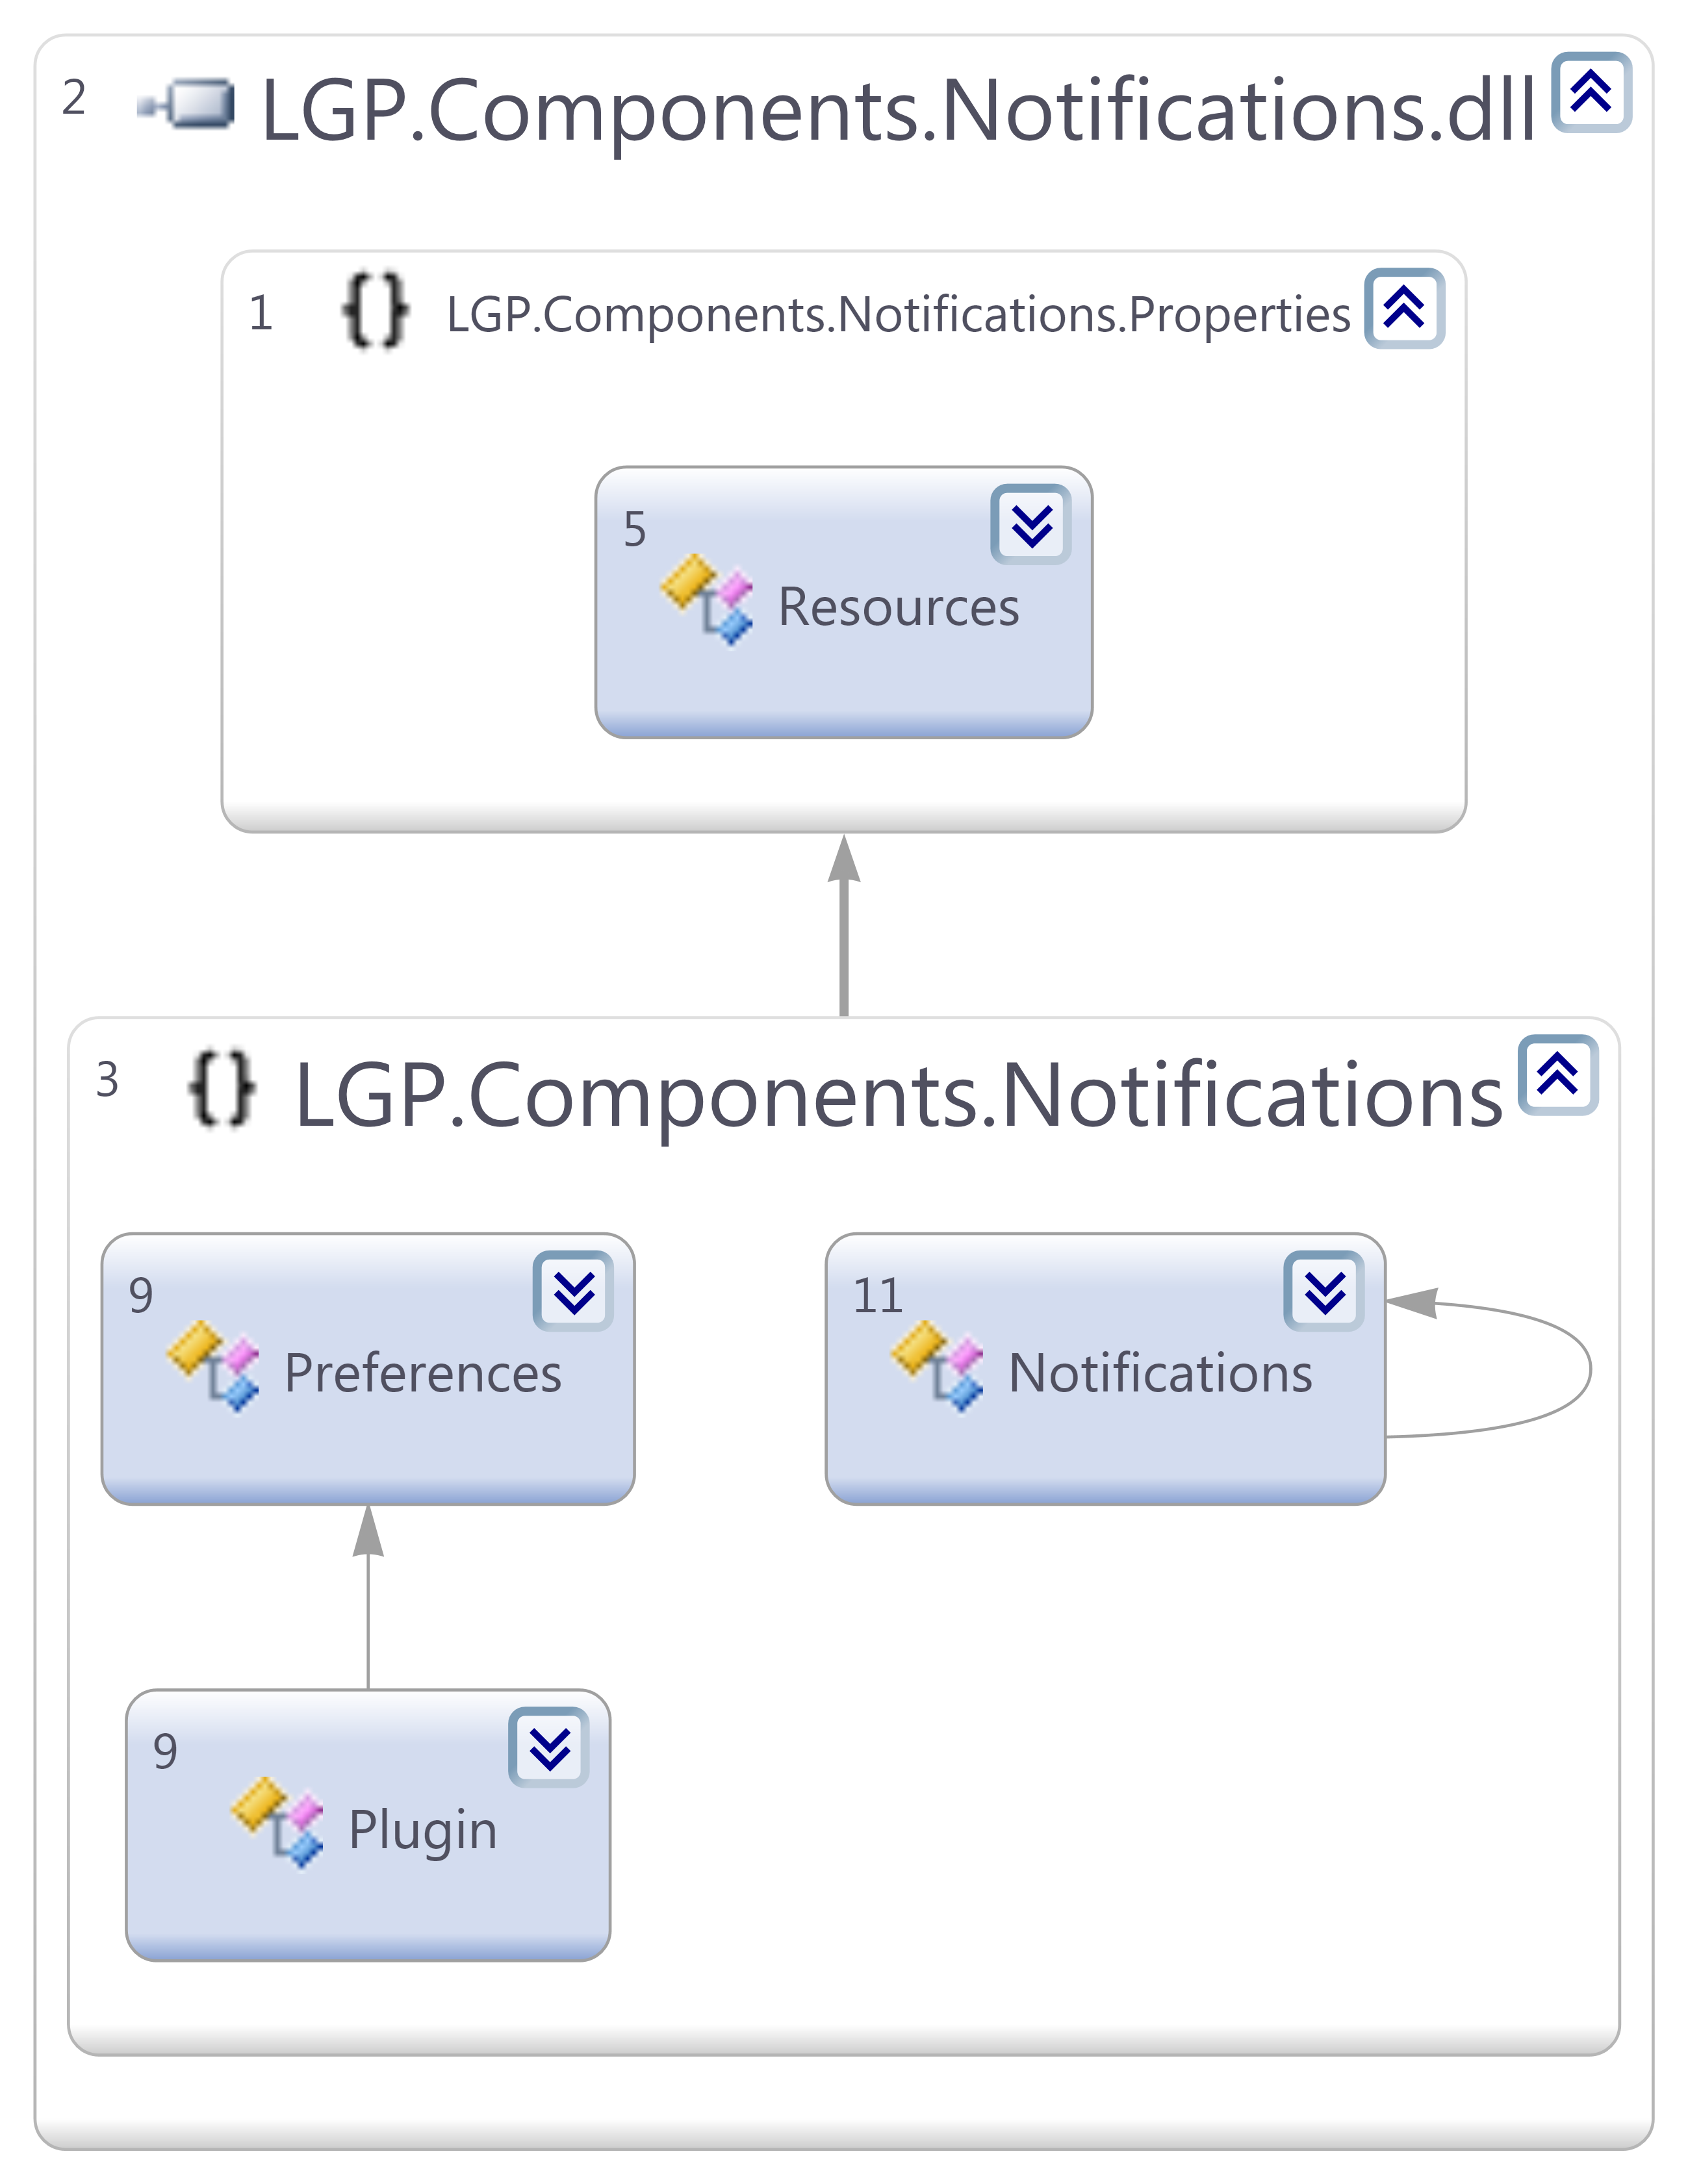
\includegraphics[scale=0.30]{pages/appendix3/figures/dllscreens/notifications.png}
				\caption{LGP.Components.Notifications}
			\end{figurehere}
	
	
		\large{\bfseries{LGP.Components.Dialog}}
		\vspace{5mm}
		
			\begin{figurehere}
				\centering
				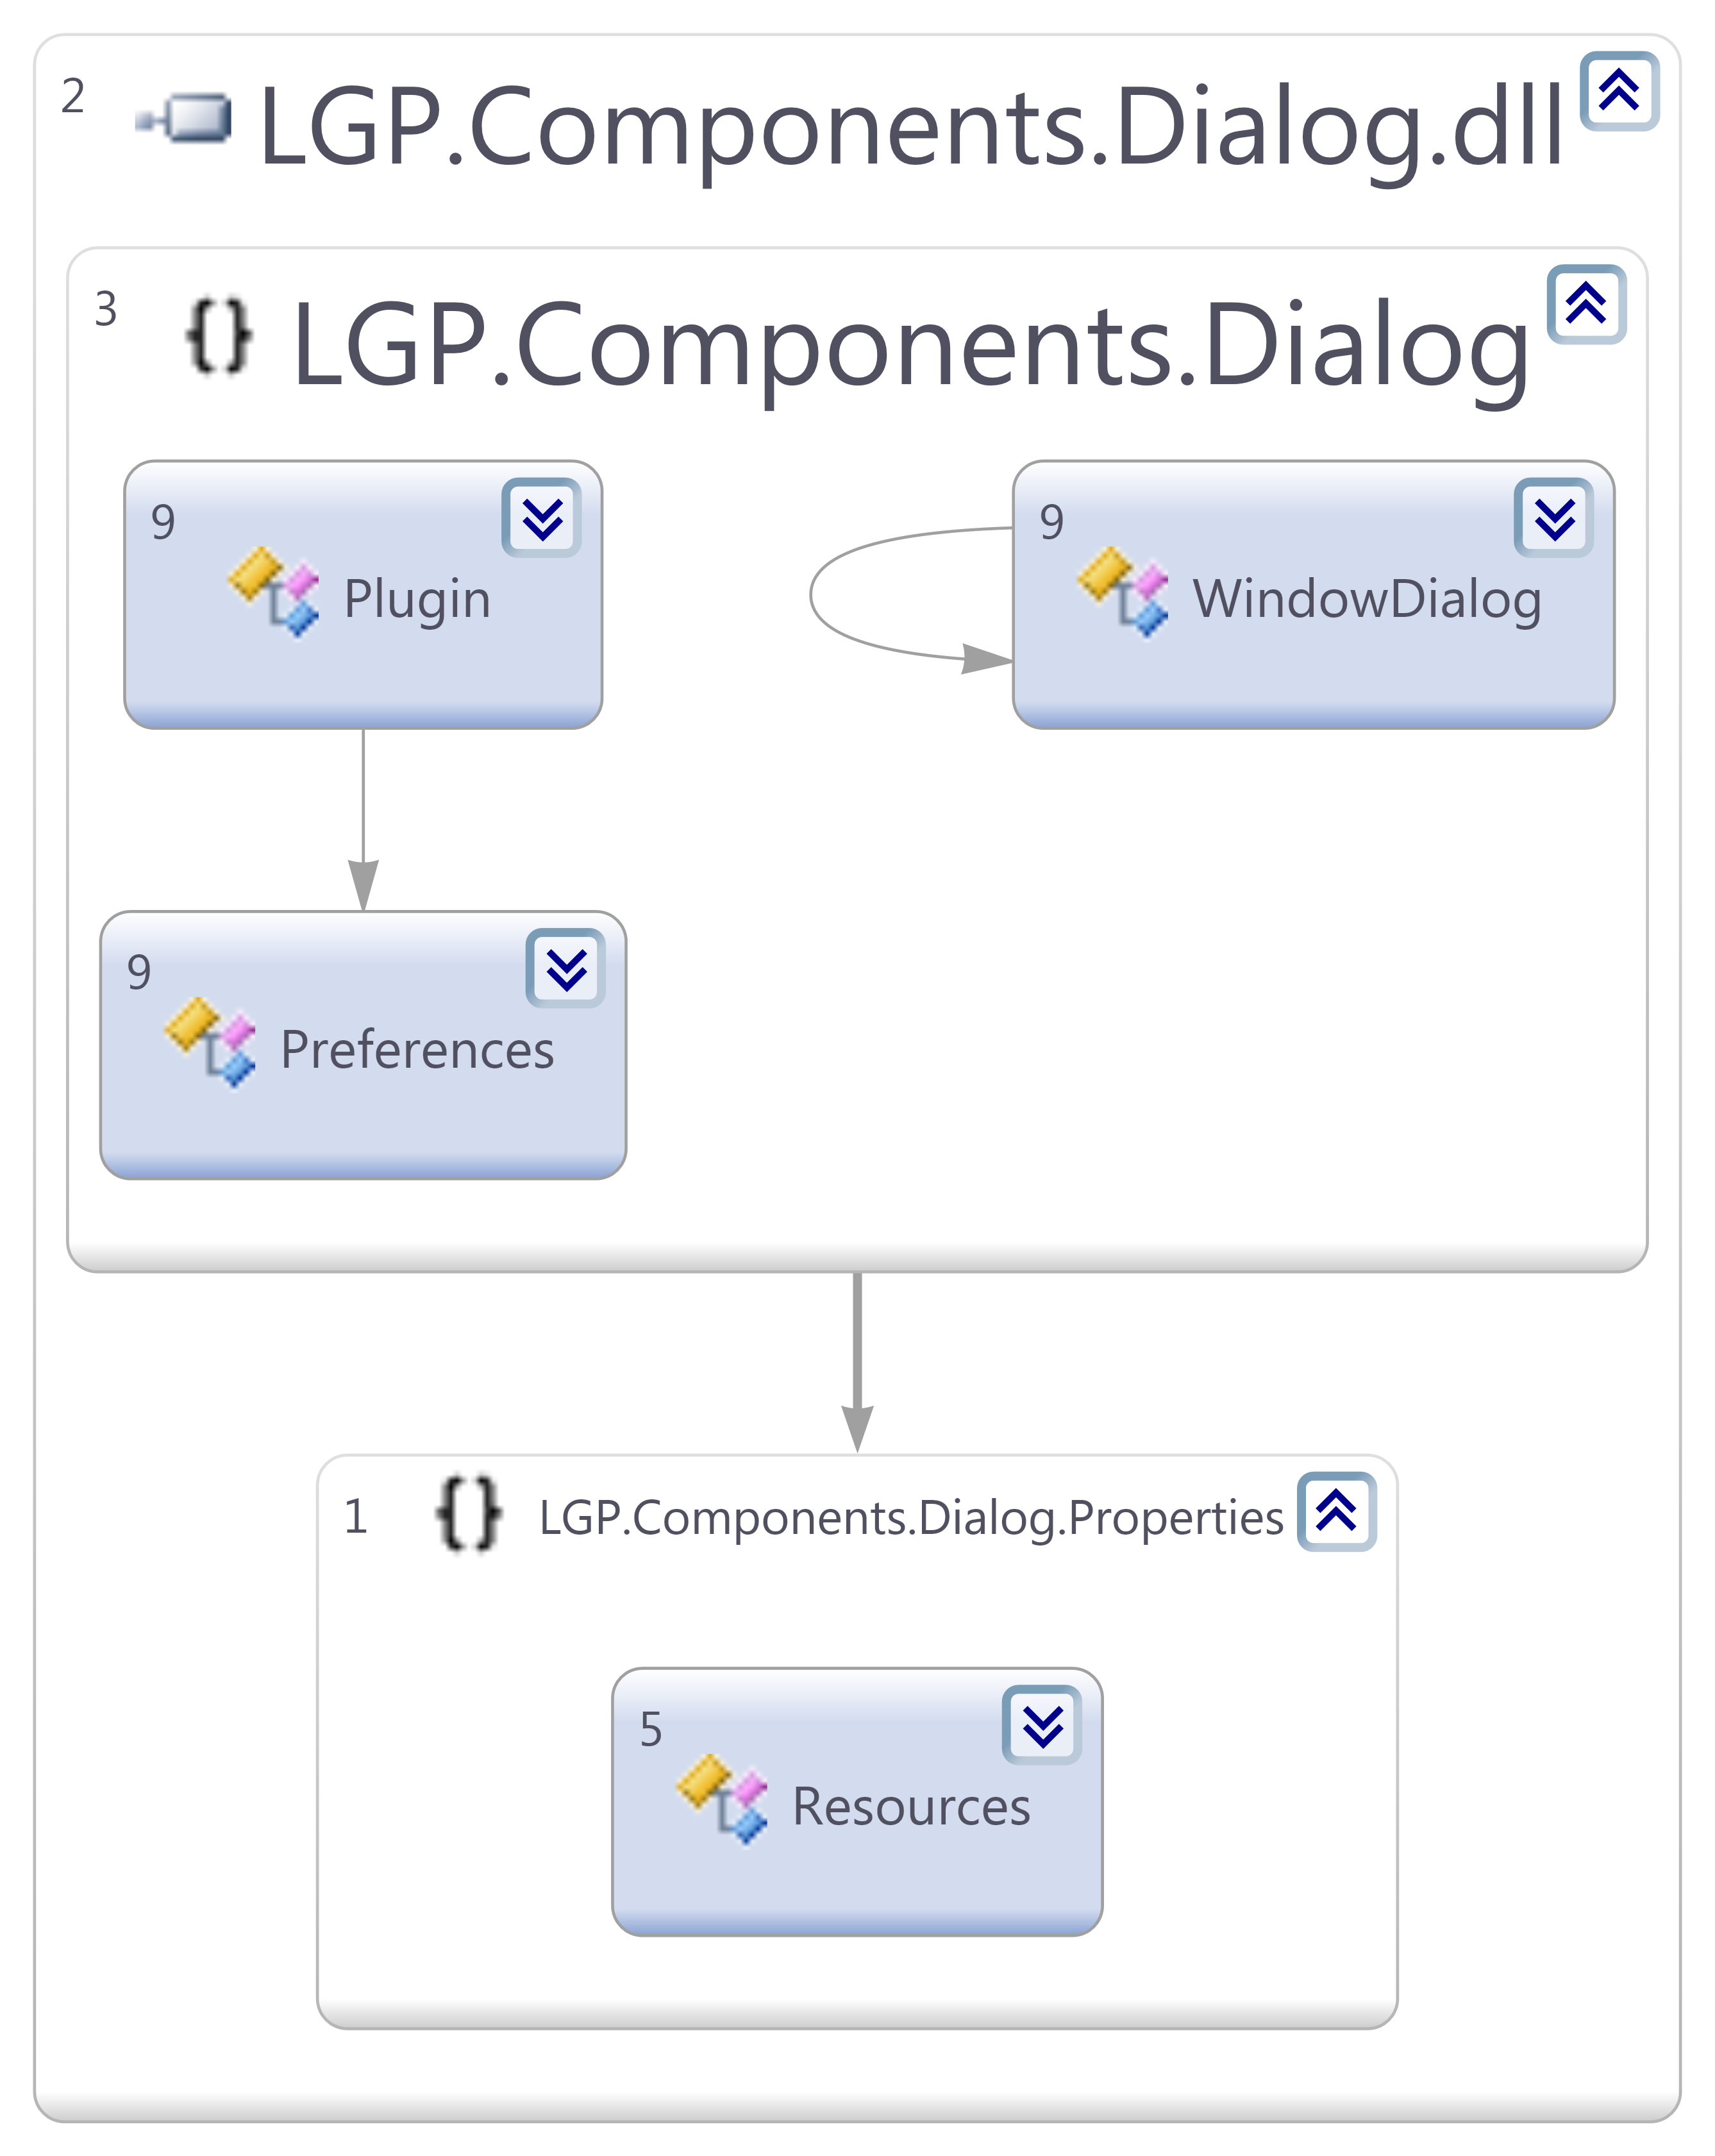
\includegraphics[scale=0.30]{pages/appendix3/figures/dllscreens/dialog.png}
				\caption{LGP.Components.Dialog}
			\end{figurehere}
		
	\columnbreak
		
		\large{\bfseries{LGP.Components.Panels}}
		\vspace{5mm}
		
			\begin{figurehere}
				\centering
				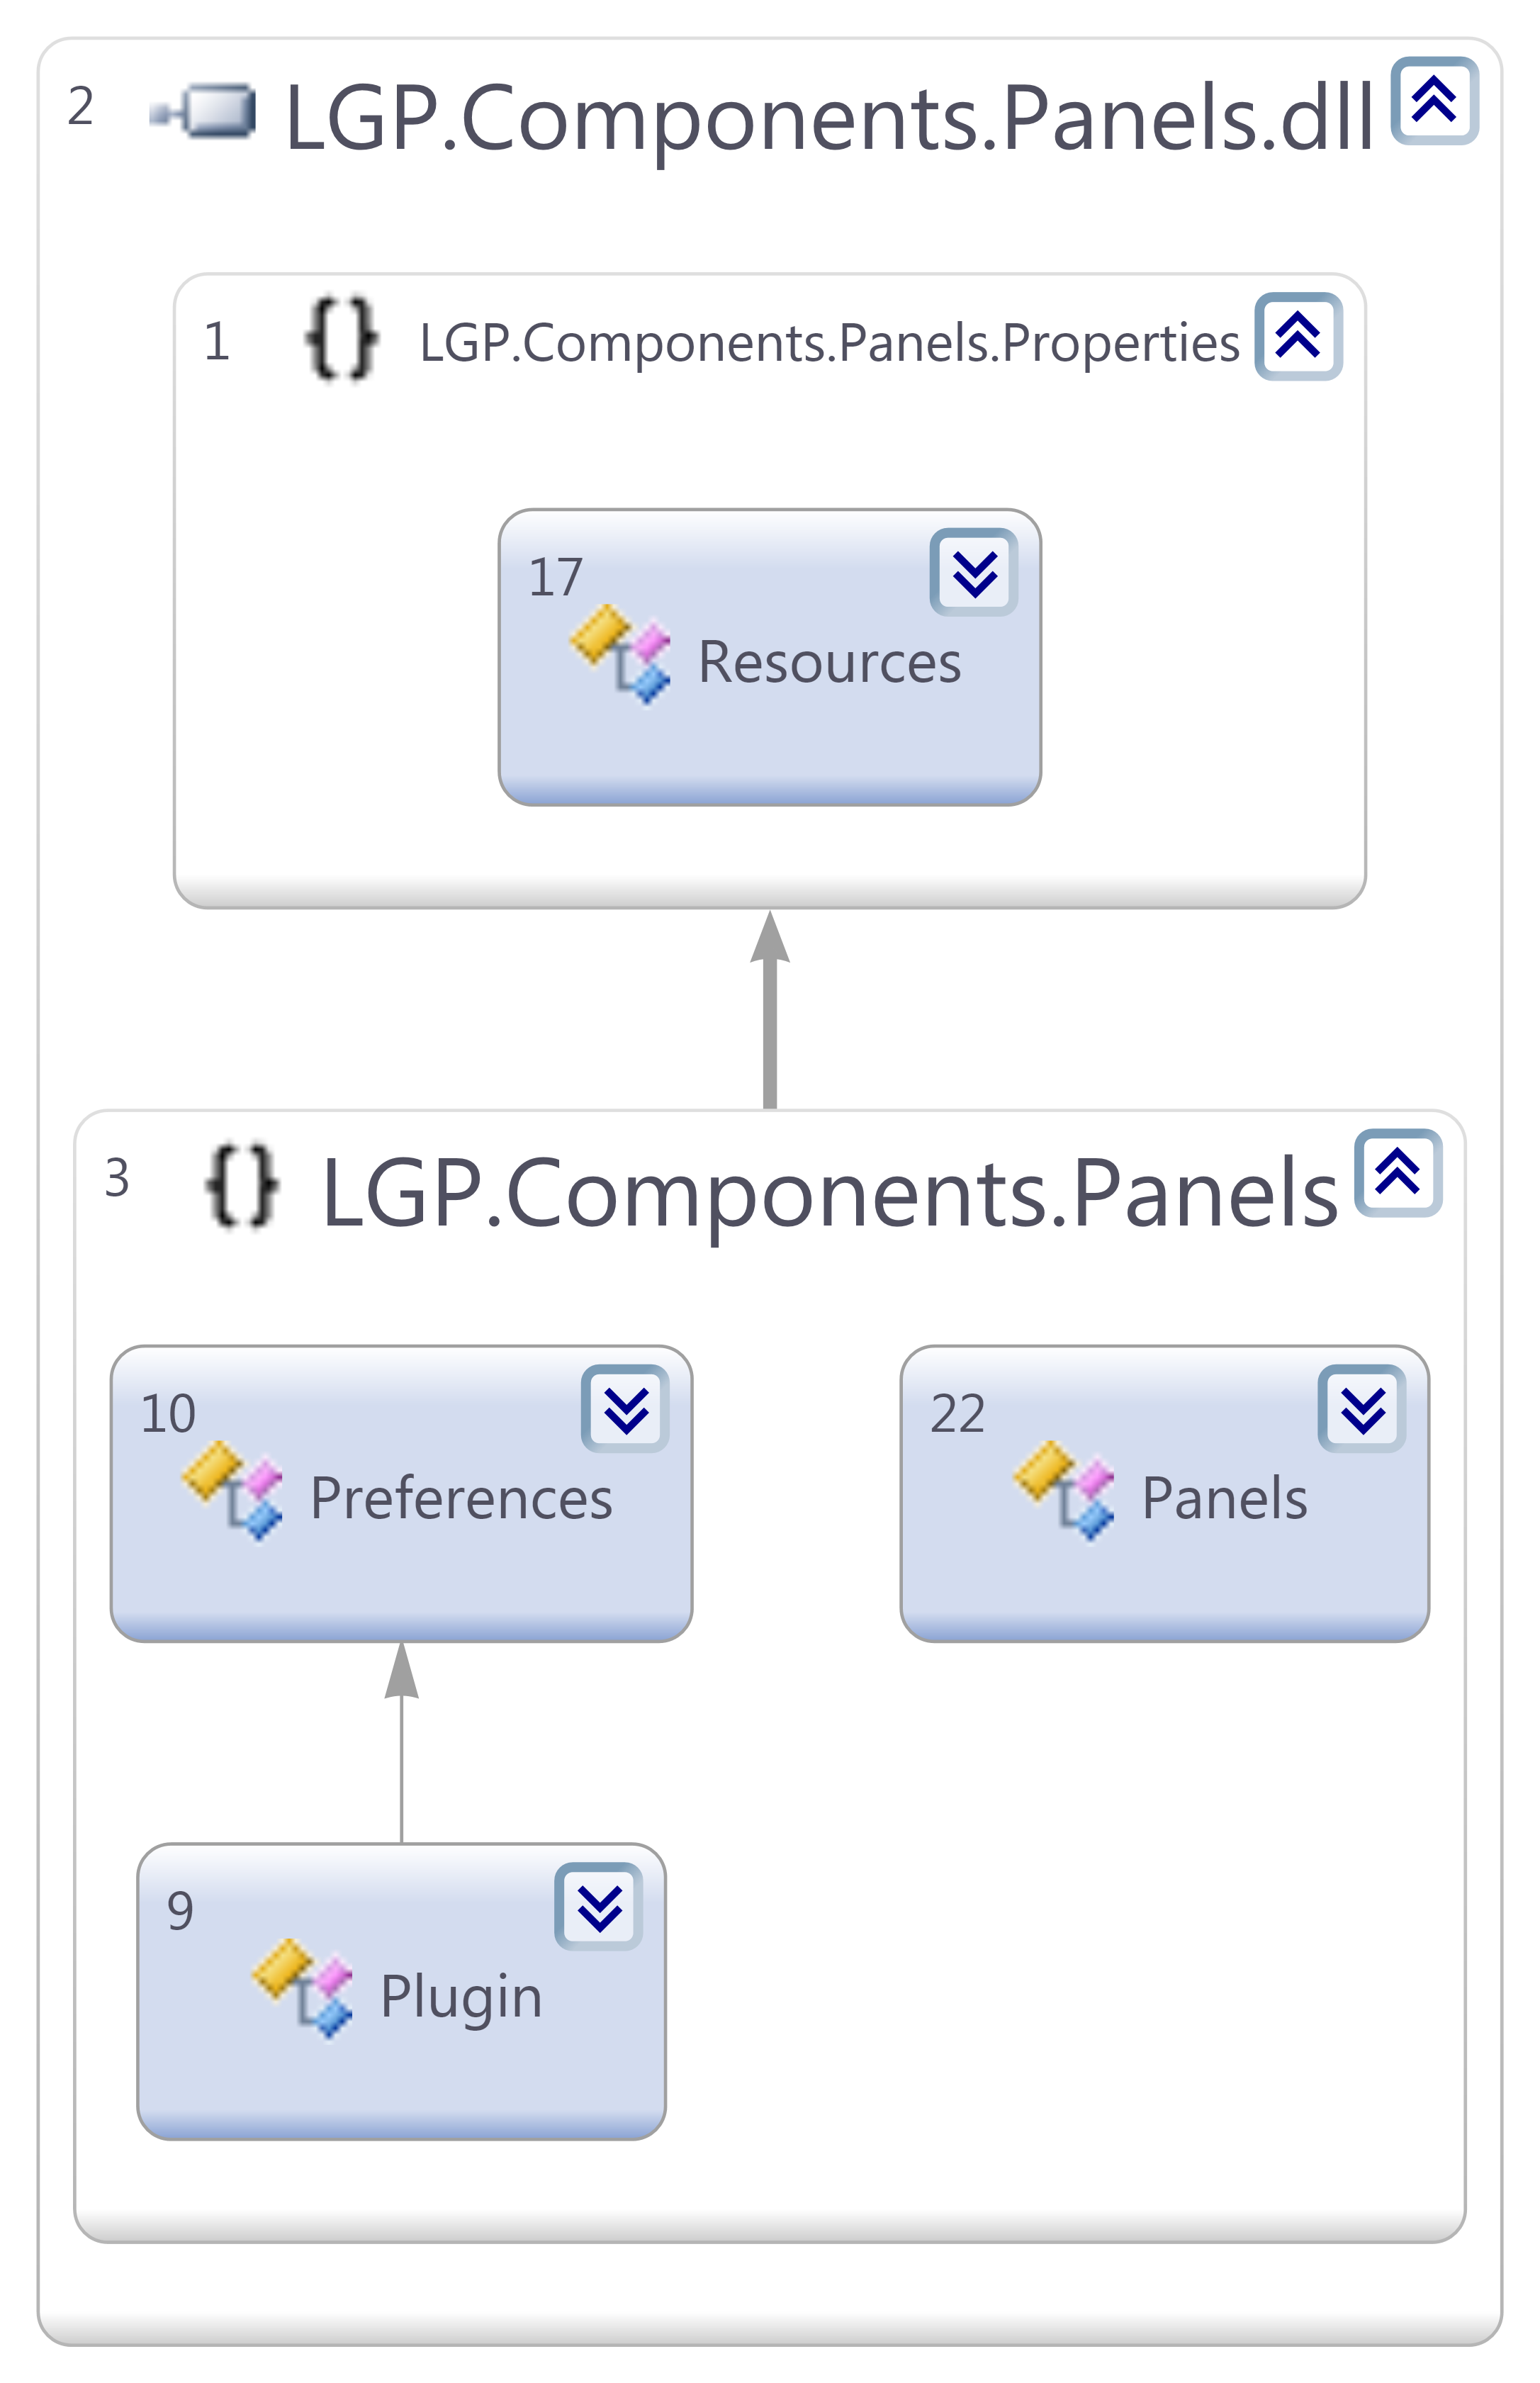
\includegraphics[scale=0.30]{pages/appendix3/figures/dllscreens/panels.png}
				\caption{LGP.Components.Panels}
			\end{figurehere}			
			
		\large{\bfseries{LGP.Components.ServerControl}}
		\vspace{5mm}
		
			\begin{figurehere}
				\centering
				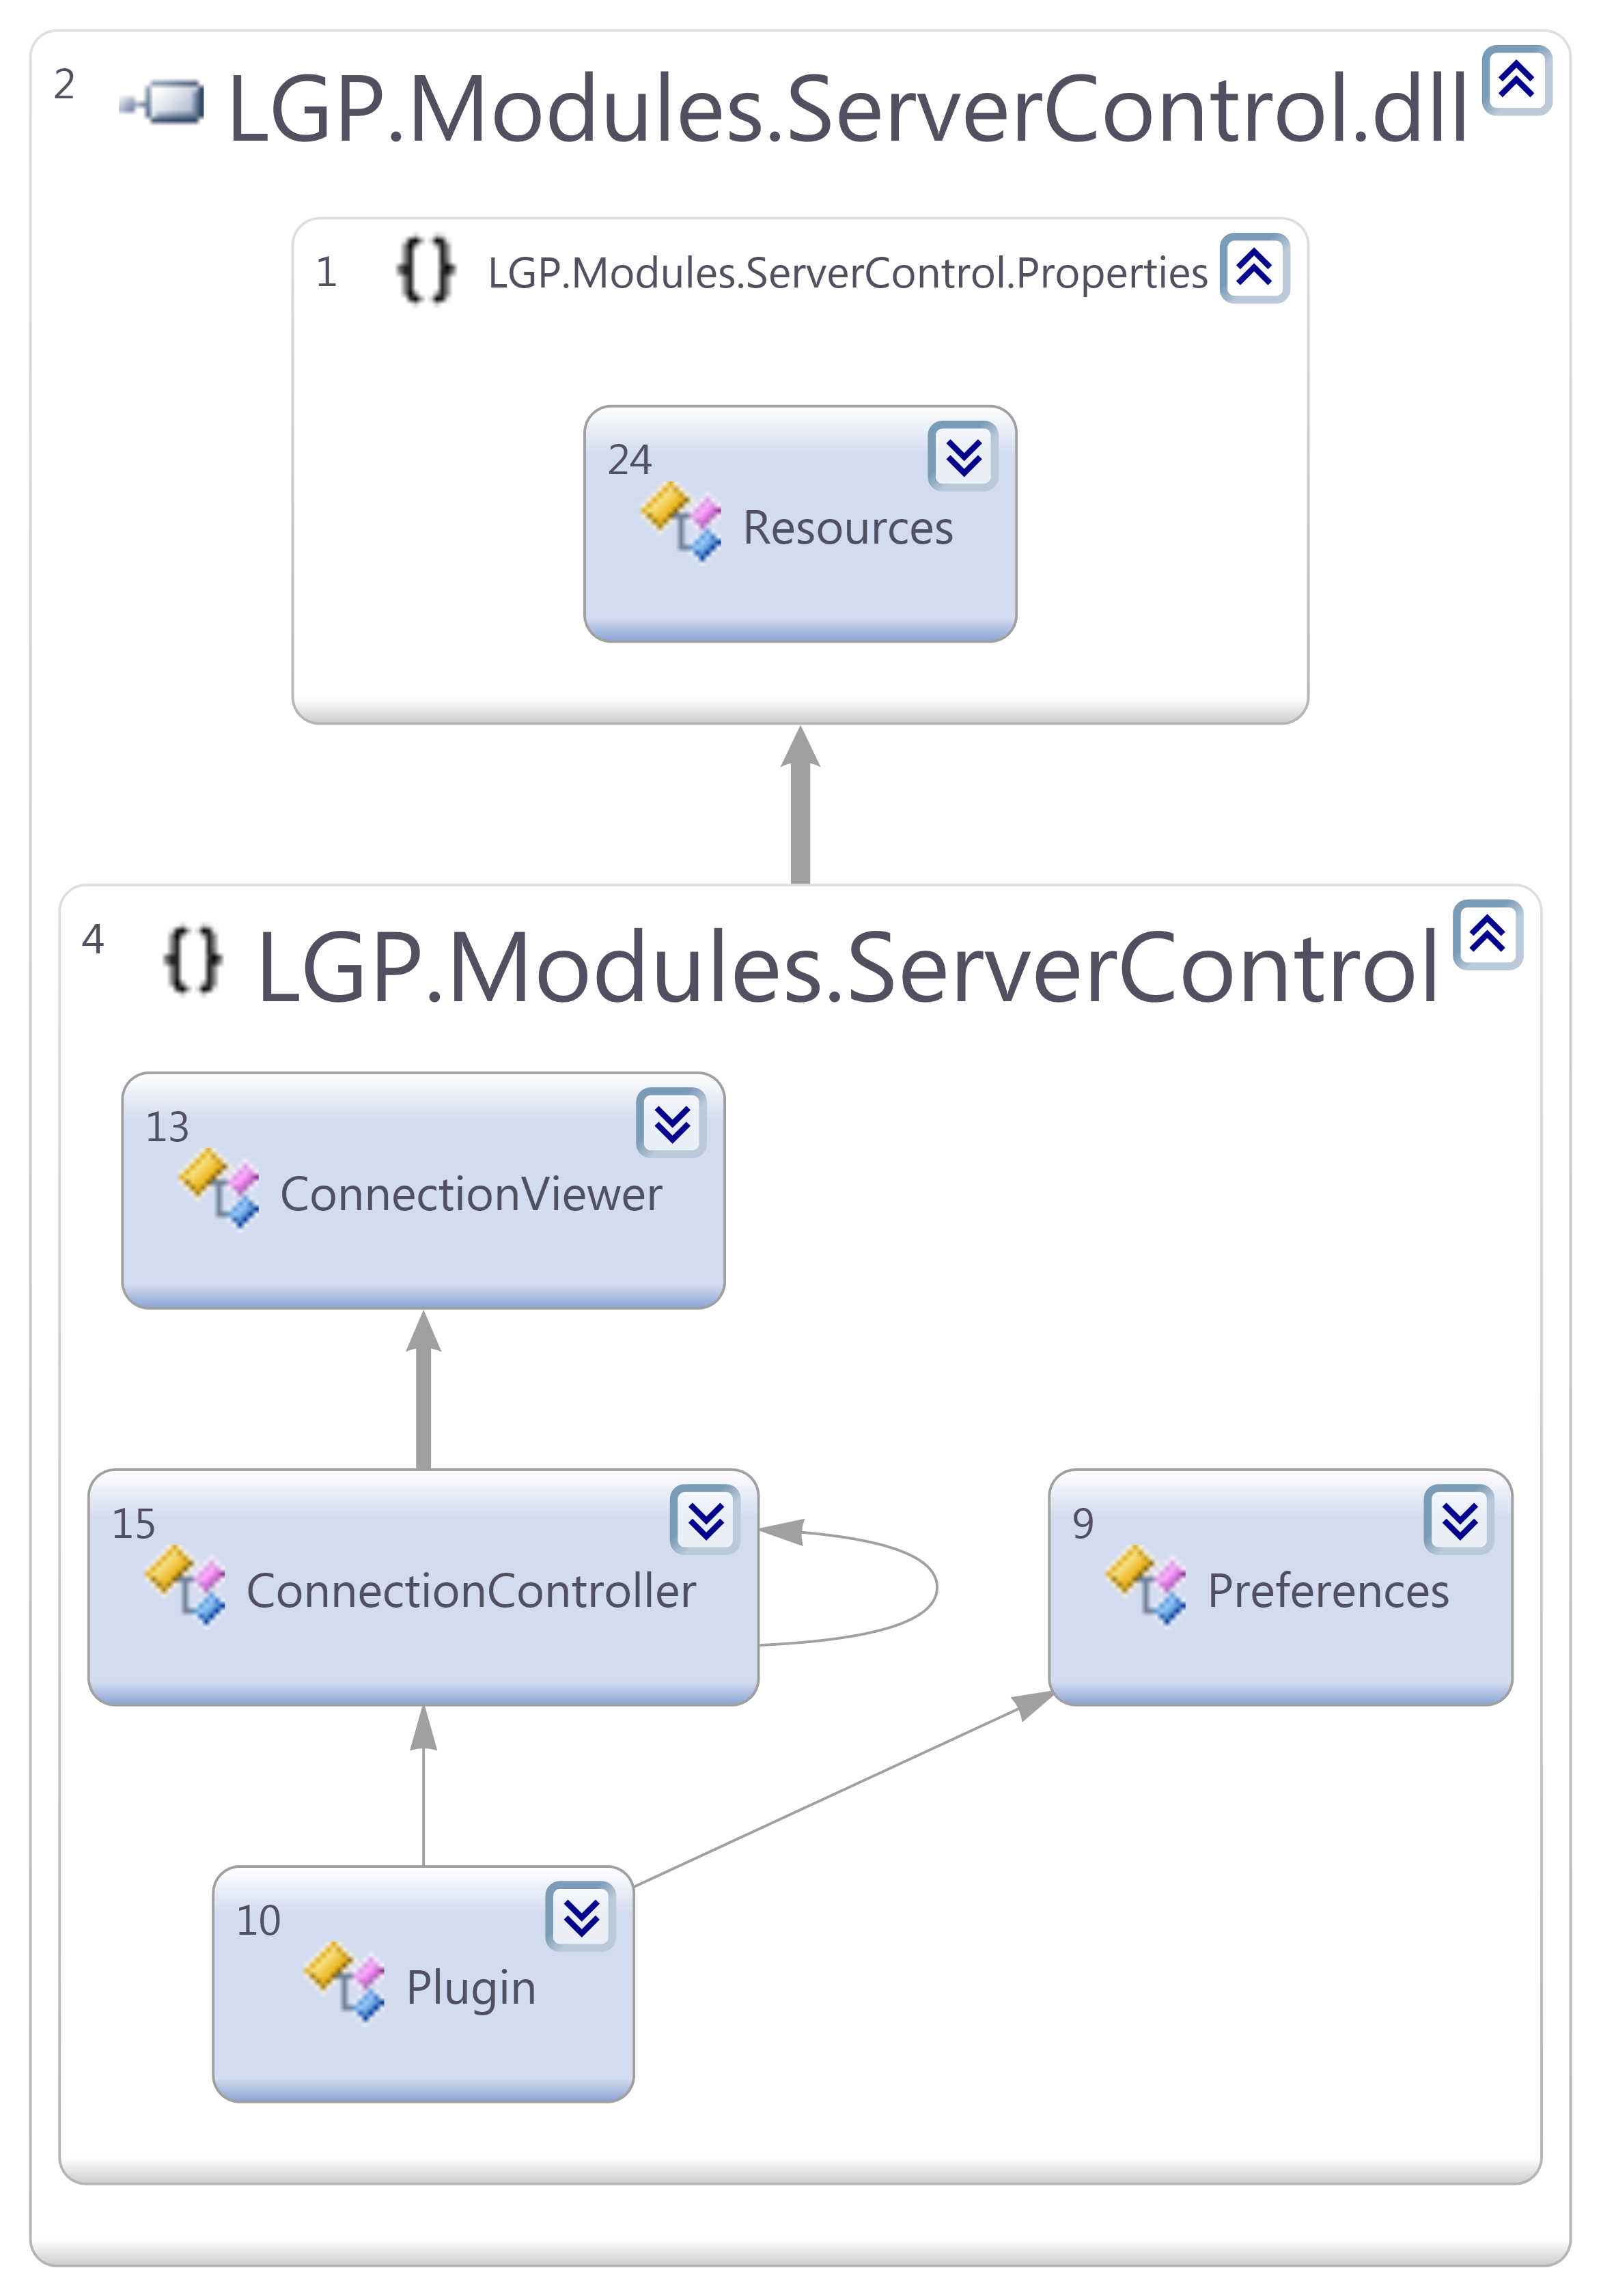
\includegraphics[scale=0.4]{pages/appendix3/figures/dllscreens/servercontrol.png}
				\caption{LGP.Modules.ServerControl}
			\end{figurehere}
	
	\end{multicols}
	
	
\newpage
	
	
	\large{\bfseries{LGP.Components.ImageLibrary}}
	\vspace{5mm}
	
		\begin{figurehere}
			\centering
			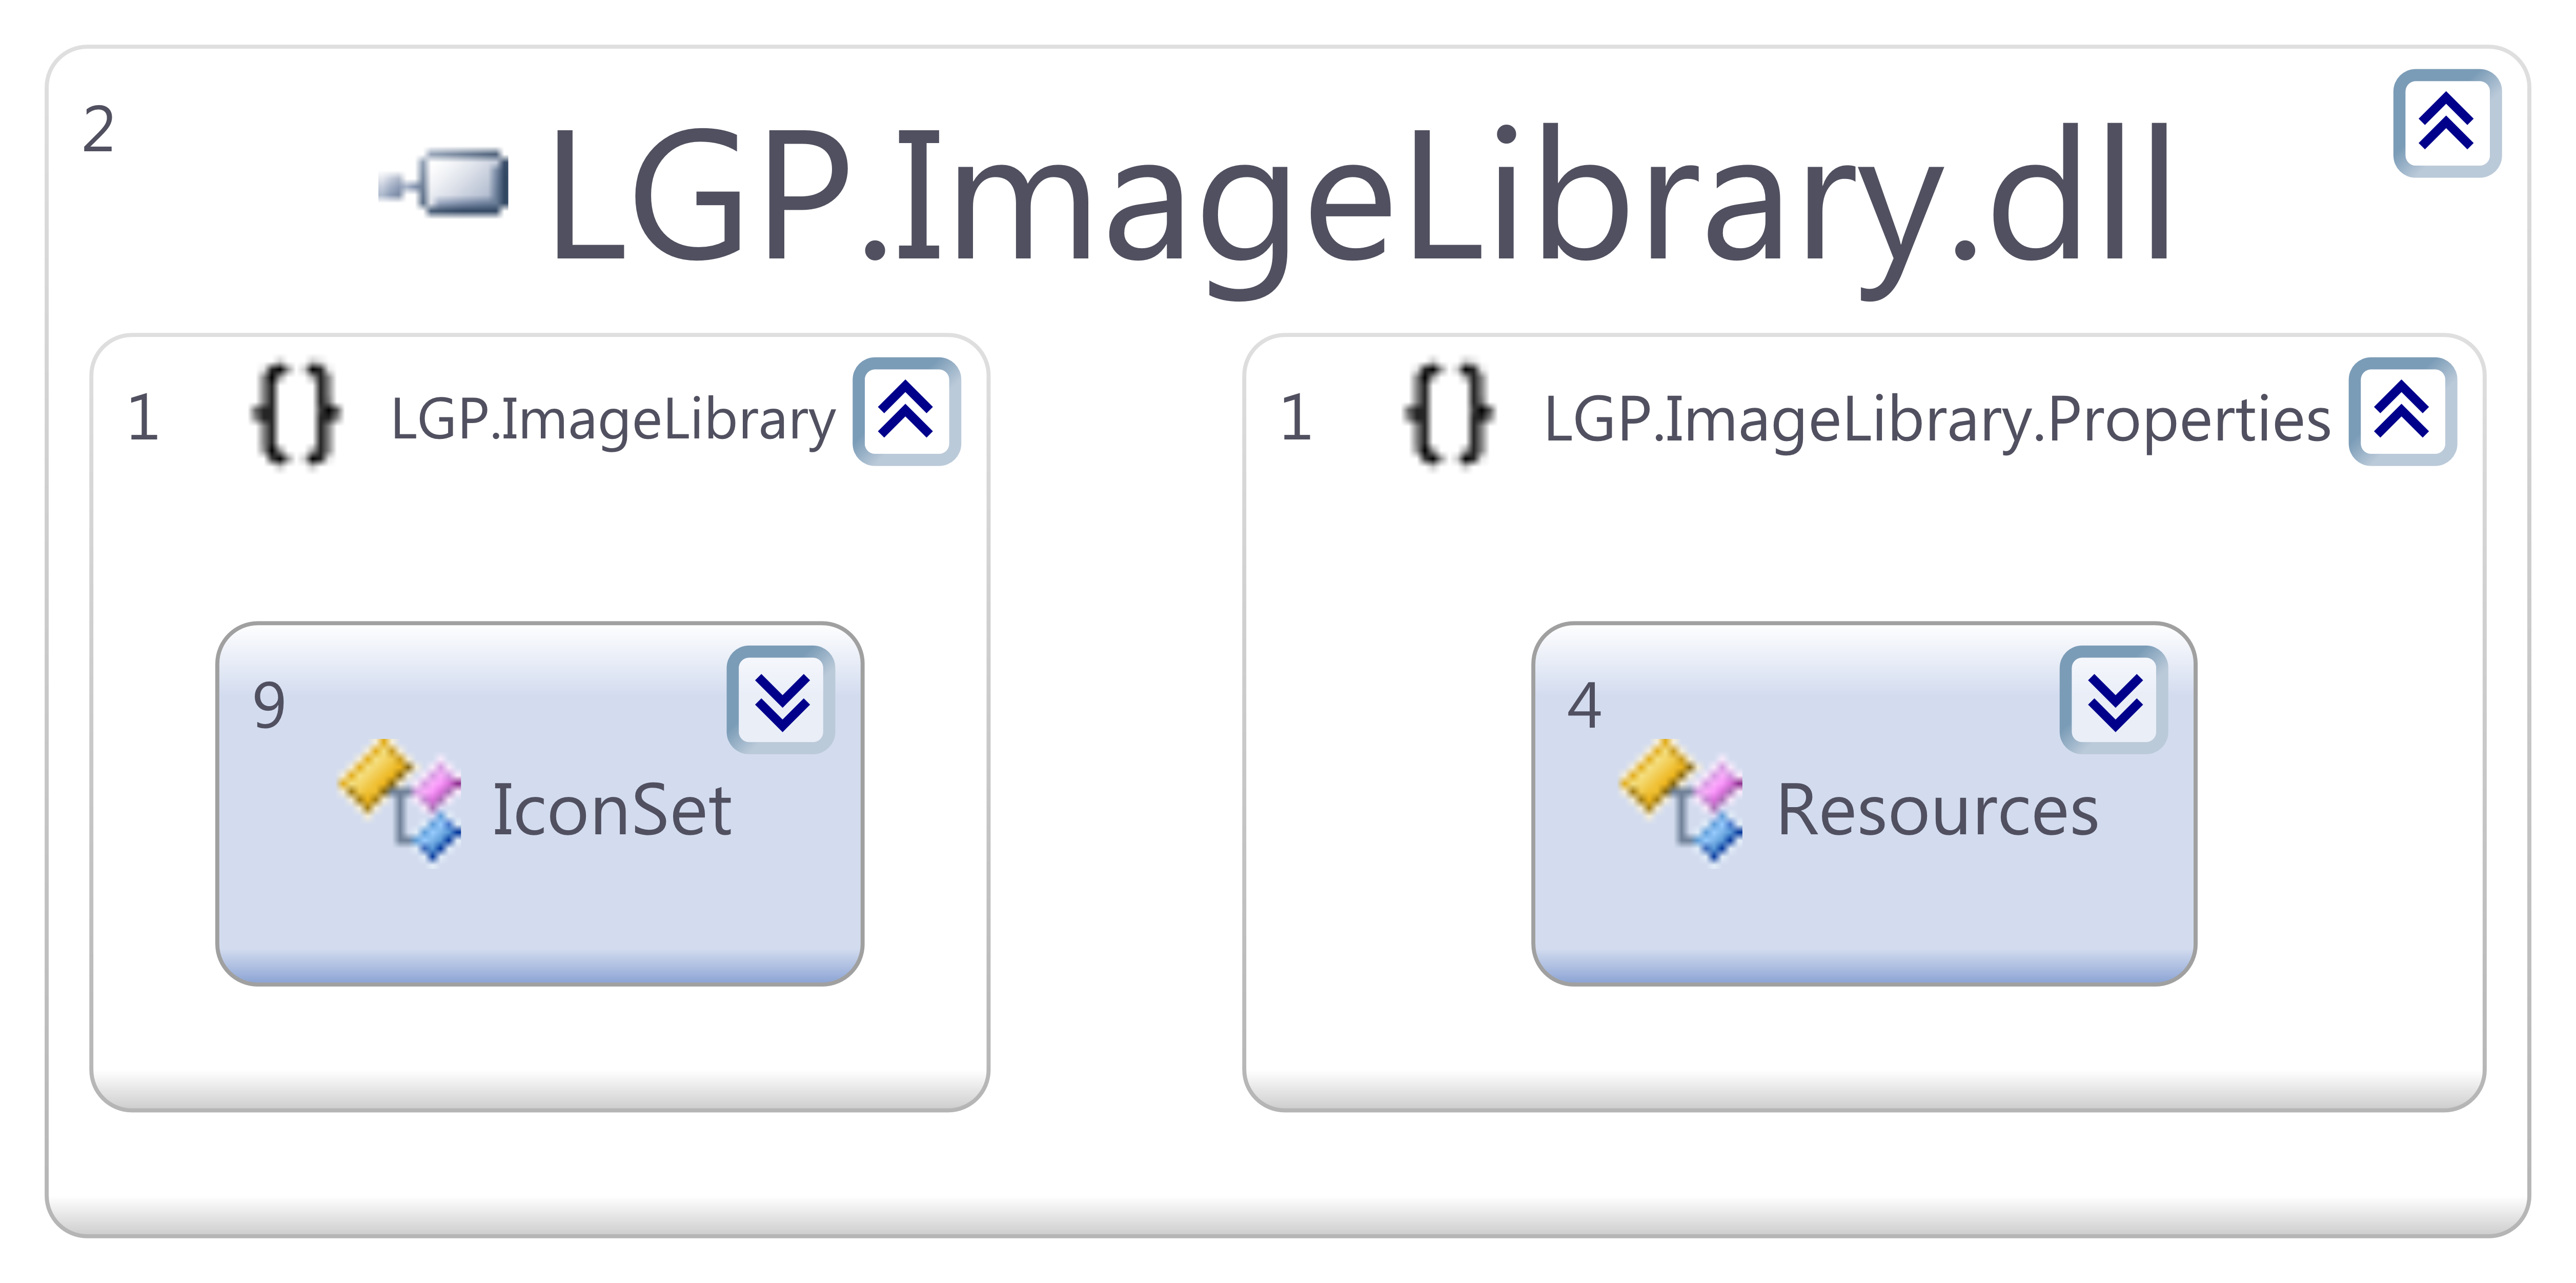
\includegraphics[scale=0.25]{pages/appendix3/figures/dllscreens/imagelibrary.png}
			\caption{LGP.ImageLibrary}
		\end{figurehere}
		

	\large{\bfseries{LGP.Components.Menus}}
	\vspace{5mm}

		\begin{figurehere}
			\centering
			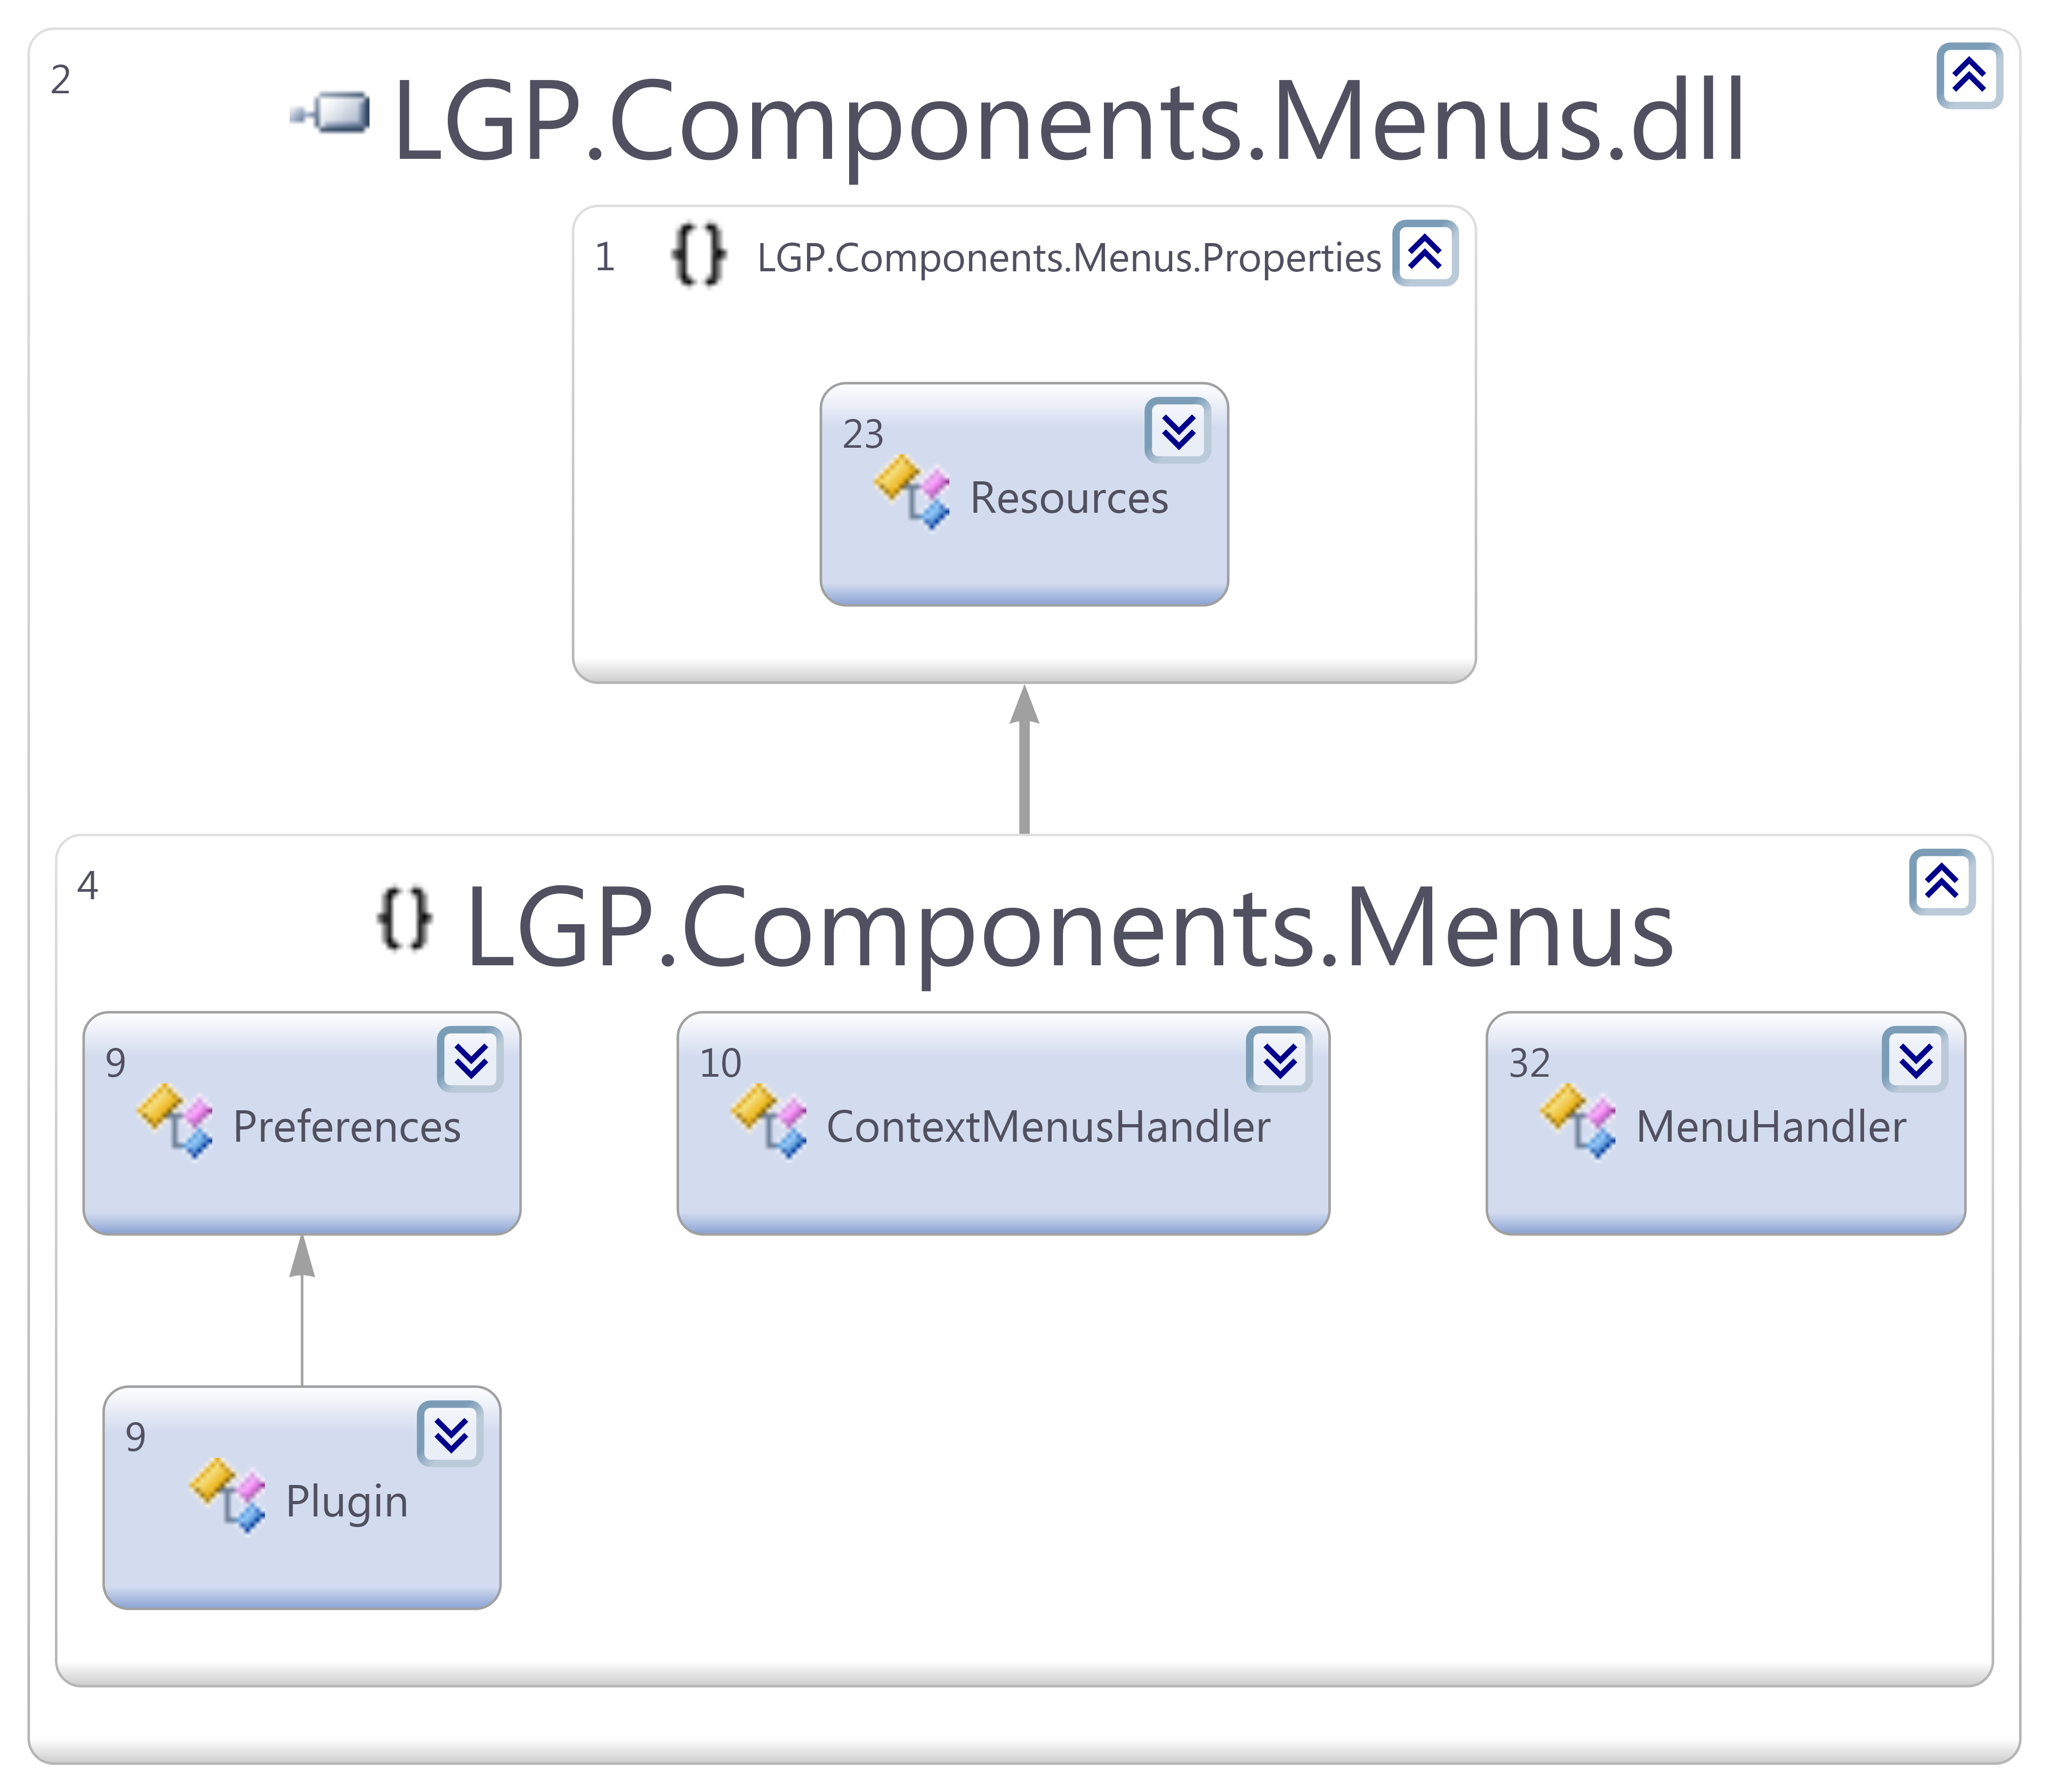
\includegraphics[scale=0.4]{pages/appendix3/figures/dllscreens/menus.png}
			\caption{LGP.Components.Menus}
		\end{figurehere}
		
		
\newpage
		
	
	\large{\bfseries{LGP.Components.Statistics}}
	\vspace{5mm}
	
		\begin{figurehere}
			\centering
			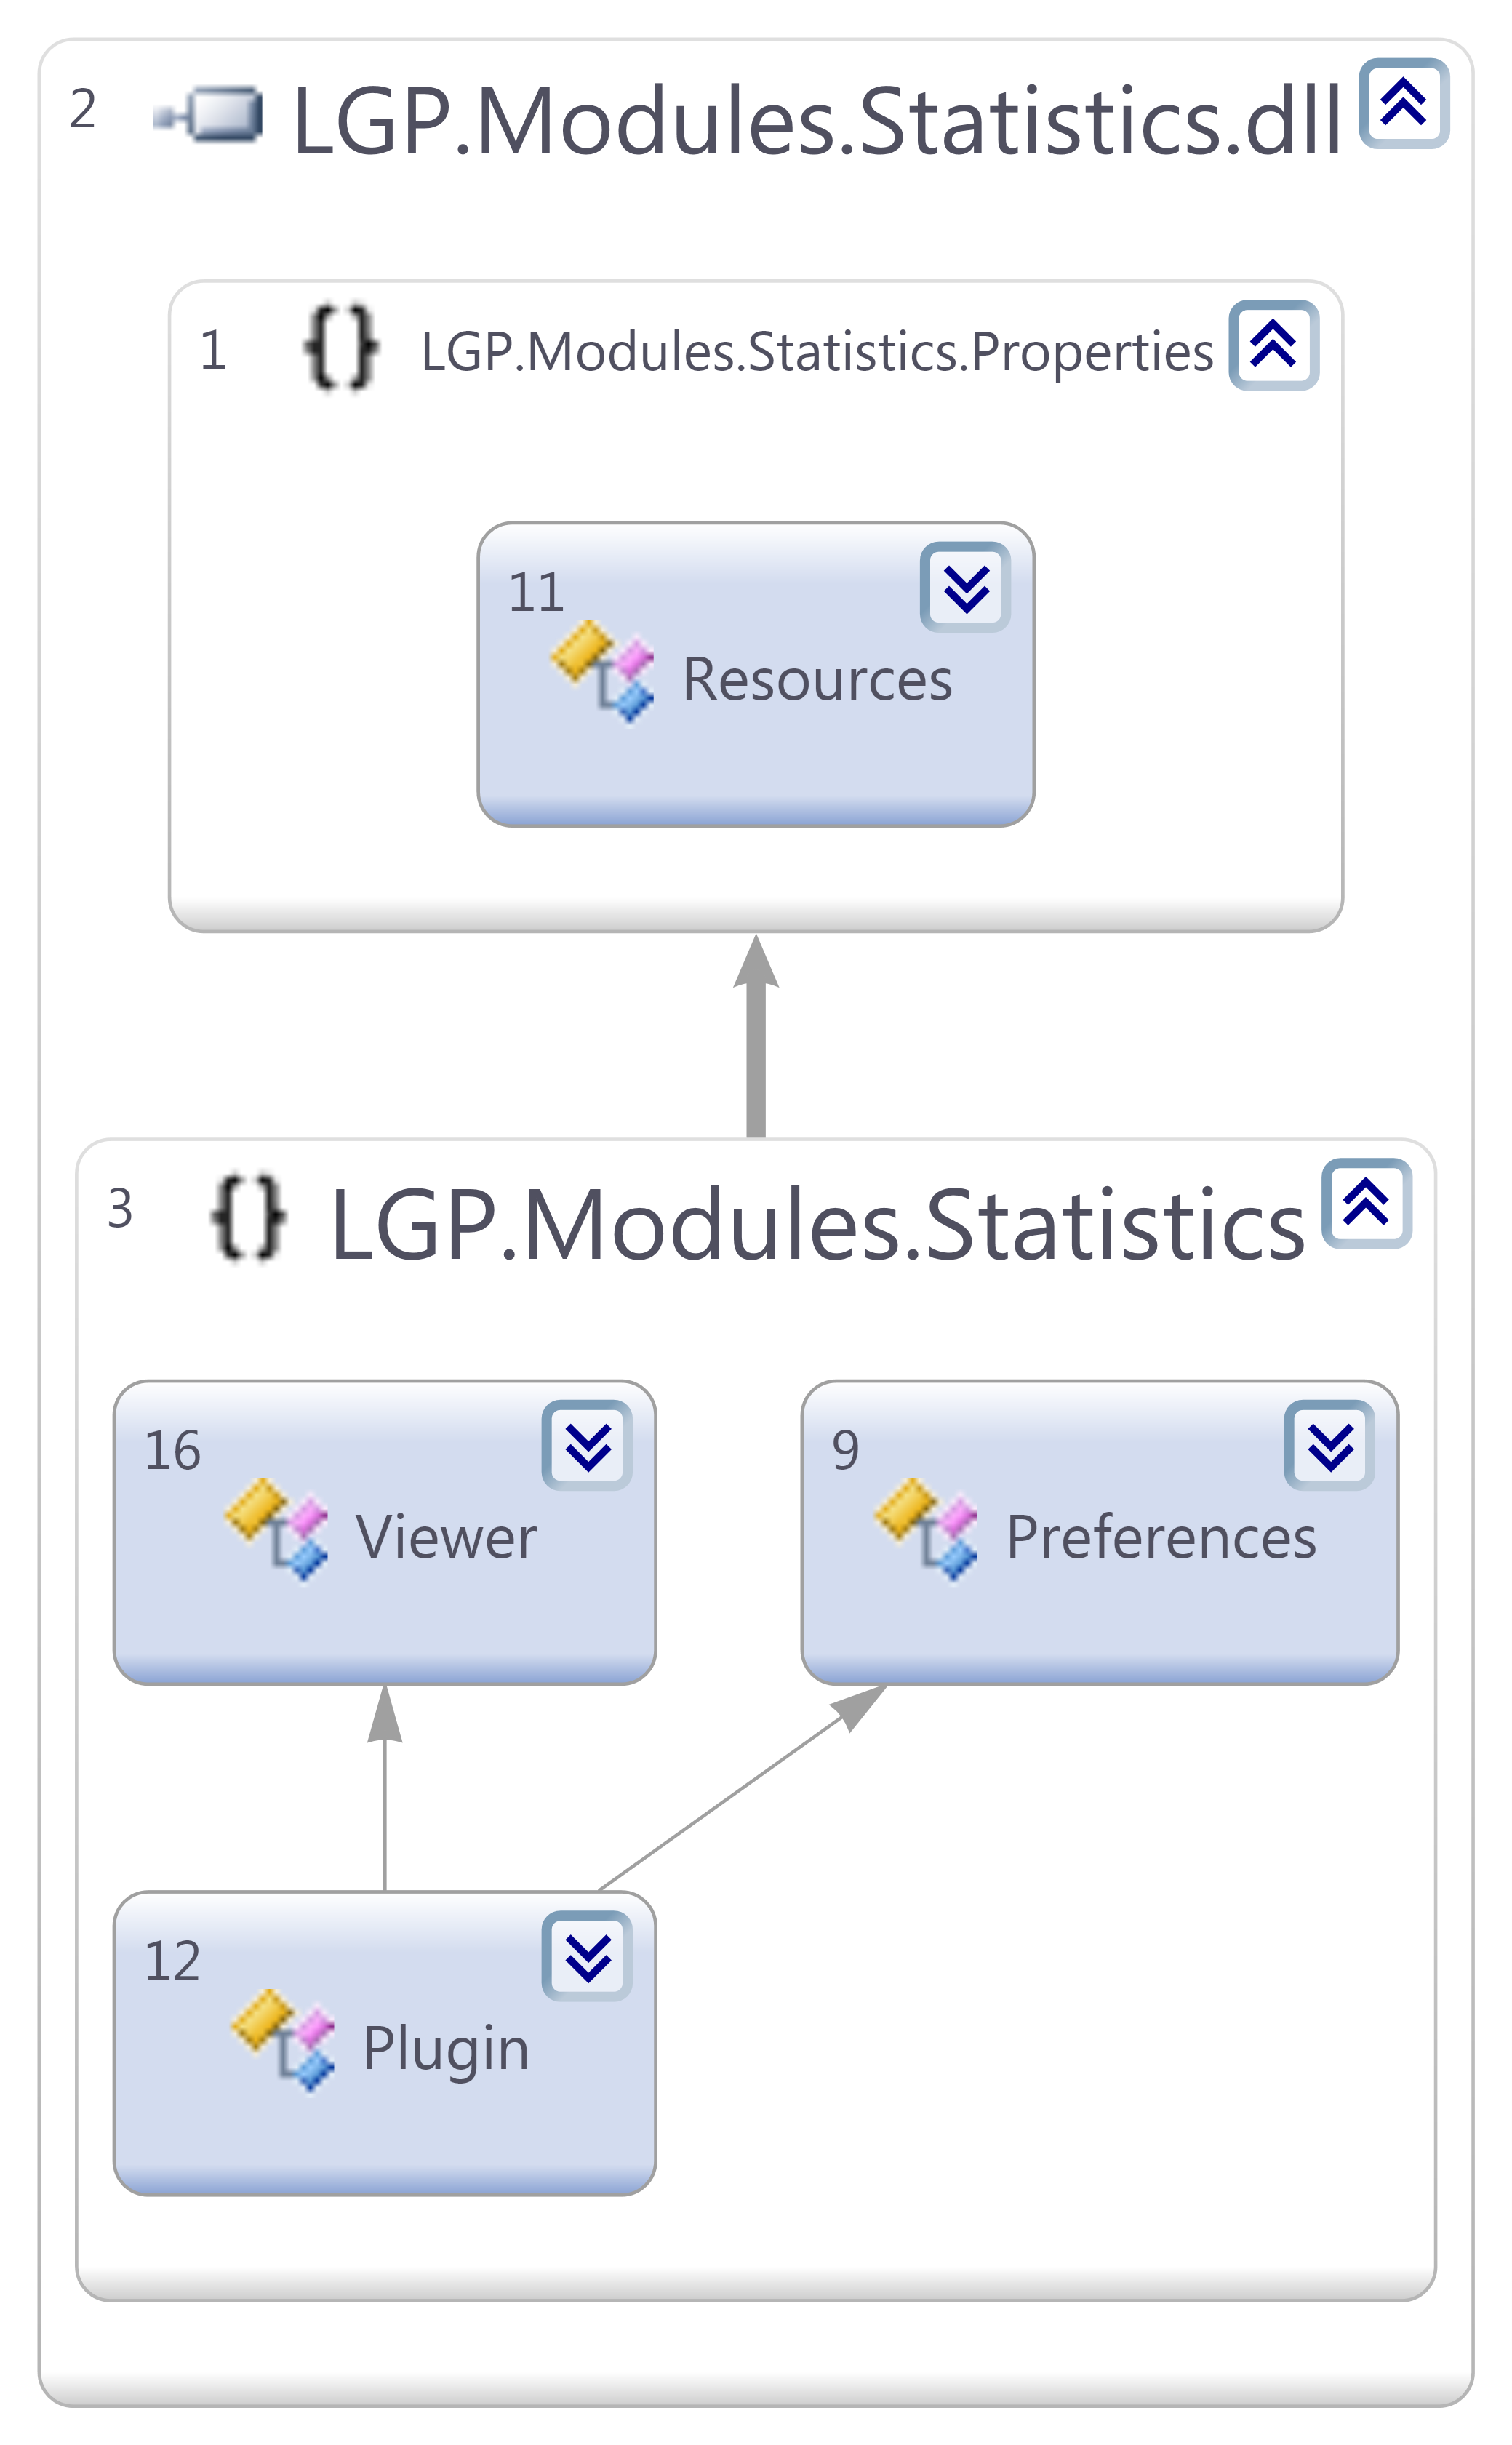
\includegraphics[scale=0.40]{pages/appendix3/figures/dllscreens/stats.png}
			\caption{LGP.Modules.Statistics}
		\end{figurehere}
		
		
\newpage
			
	
	\large{\bfseries{LGP.Components.PolicyEditor}}
	\vspace{5mm}
	
		\begin{figurehere}
			\centering
			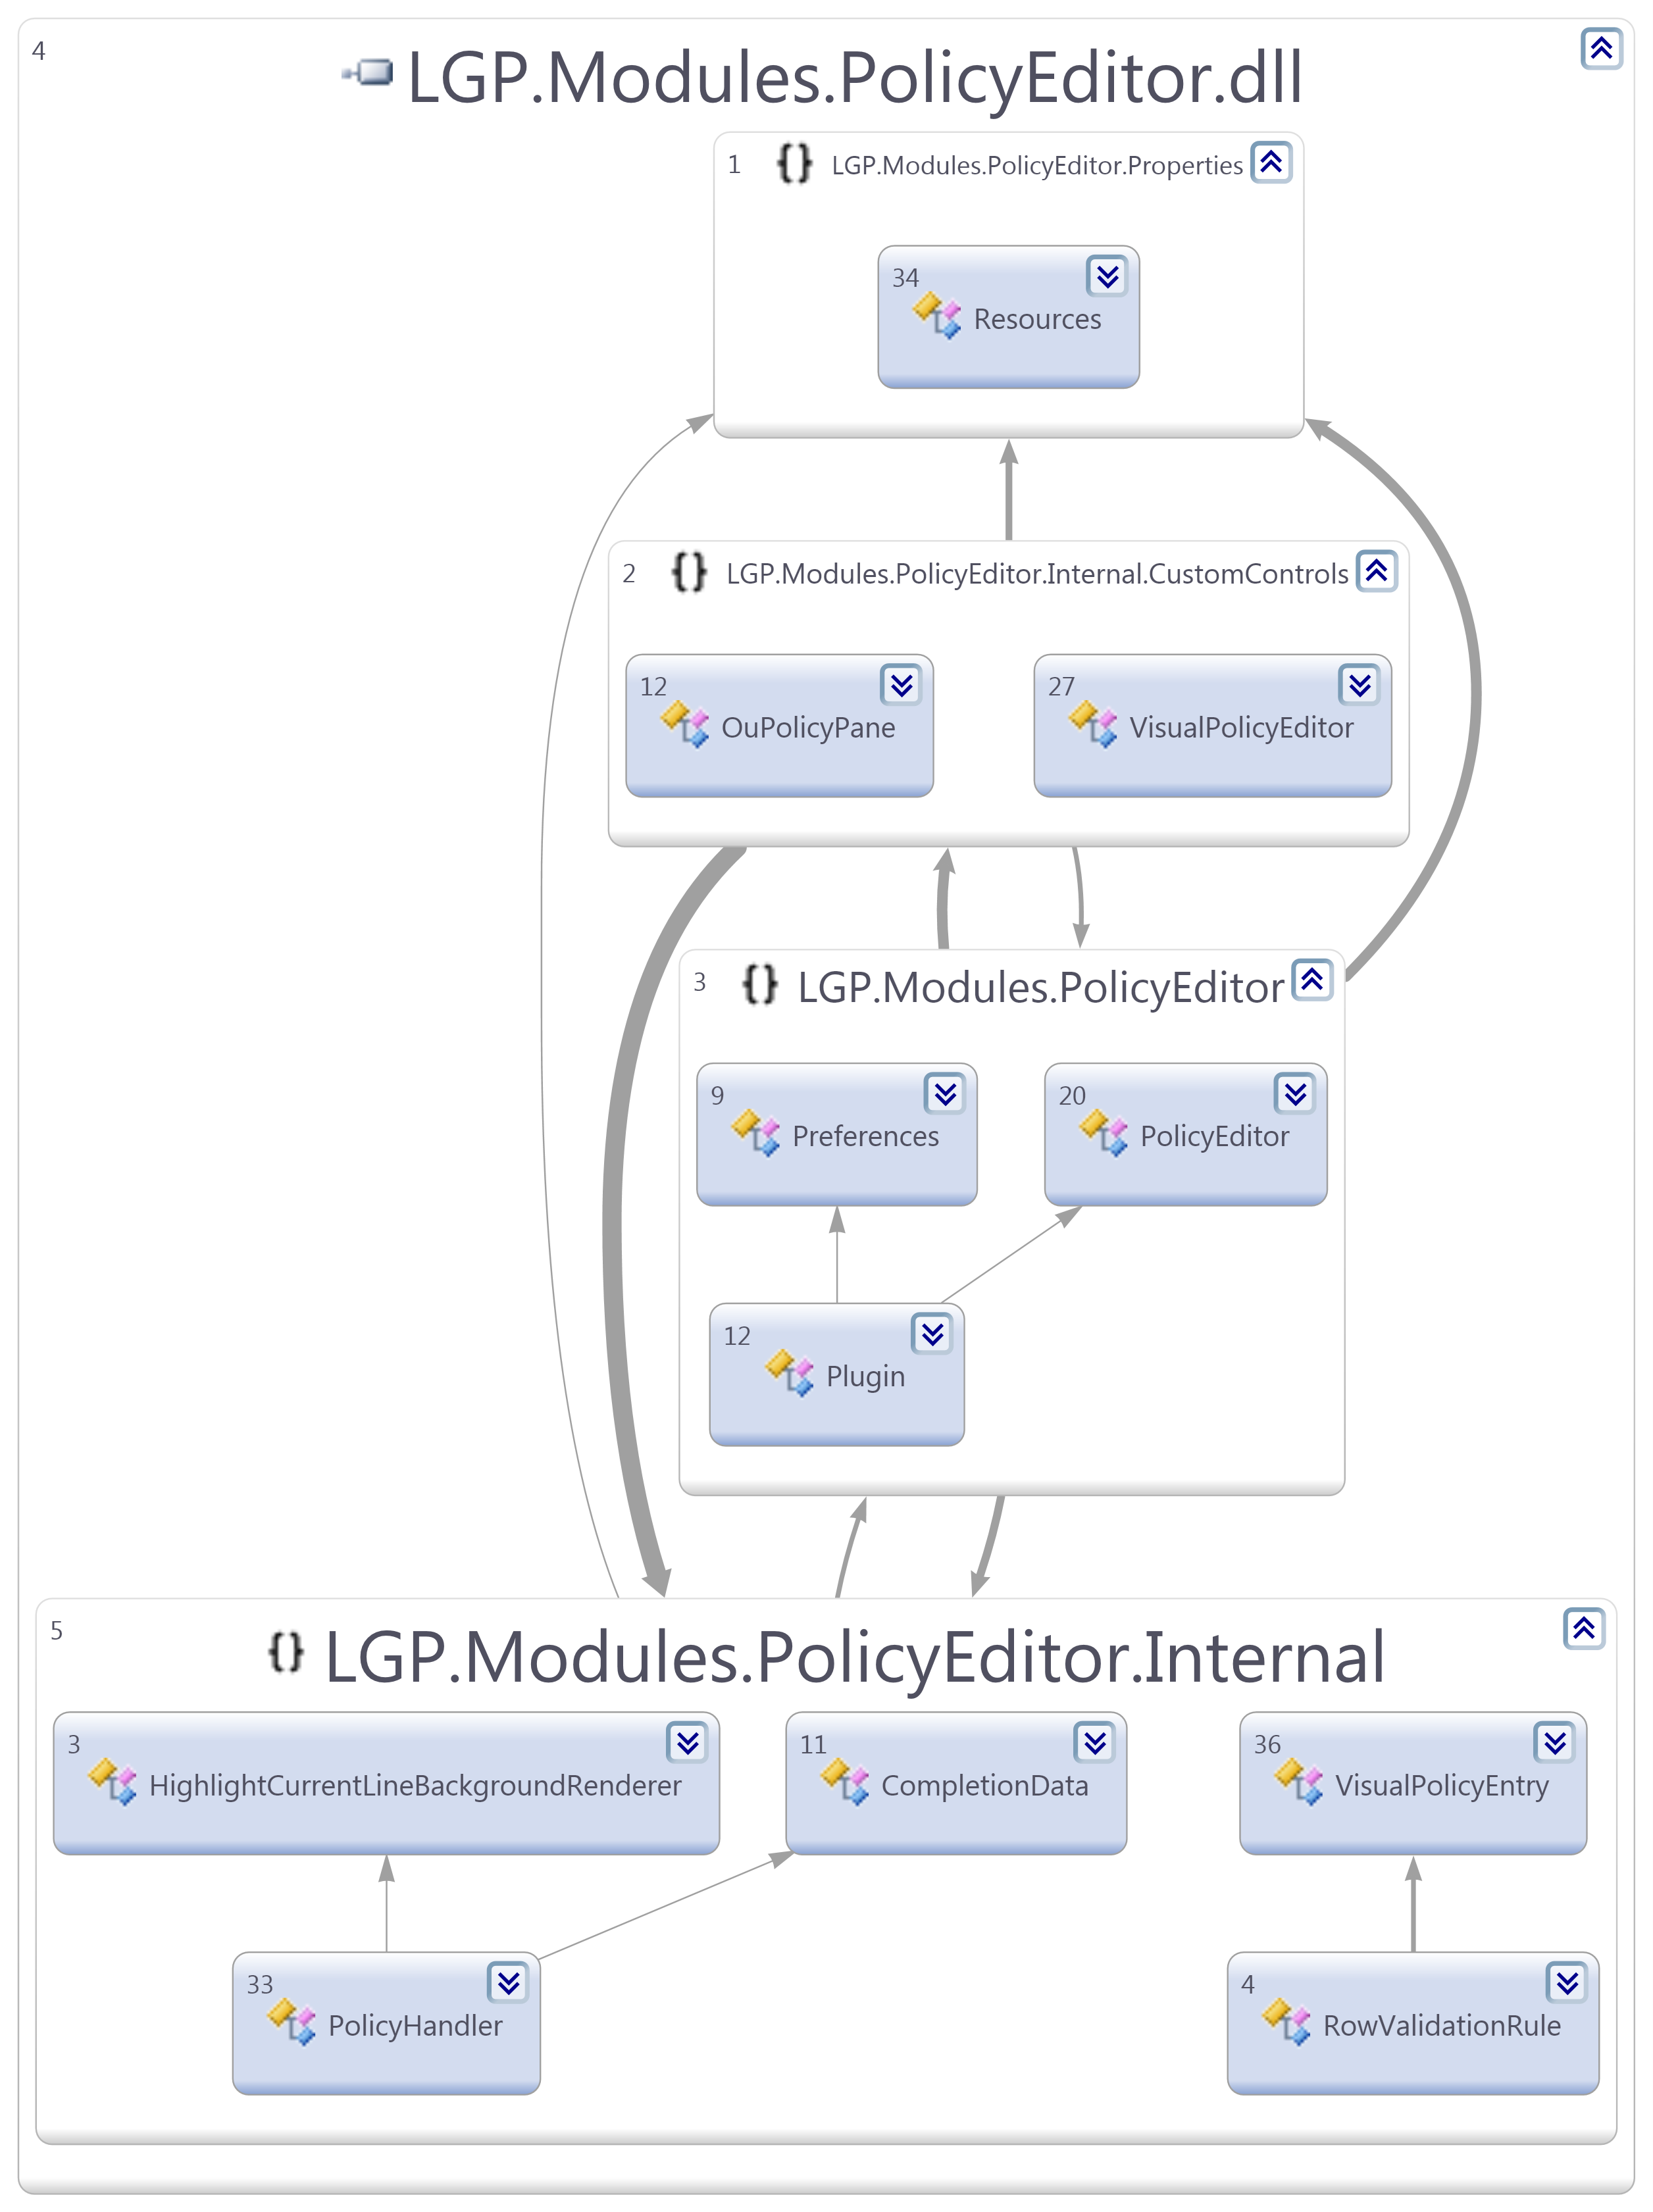
\includegraphics[scale=0.70]{pages/appendix3/figures/dllscreens/policyeditor.png}
			\caption{LGP.Modules.PolicyEditor}
		\end{figurehere}
		
		
\newpage
	
	
	\large{\bfseries{LGP.Components.OrganizationalUnitExplorer}}
	\vspace{5mm}
	
		\begin{figurehere}
			\centering
			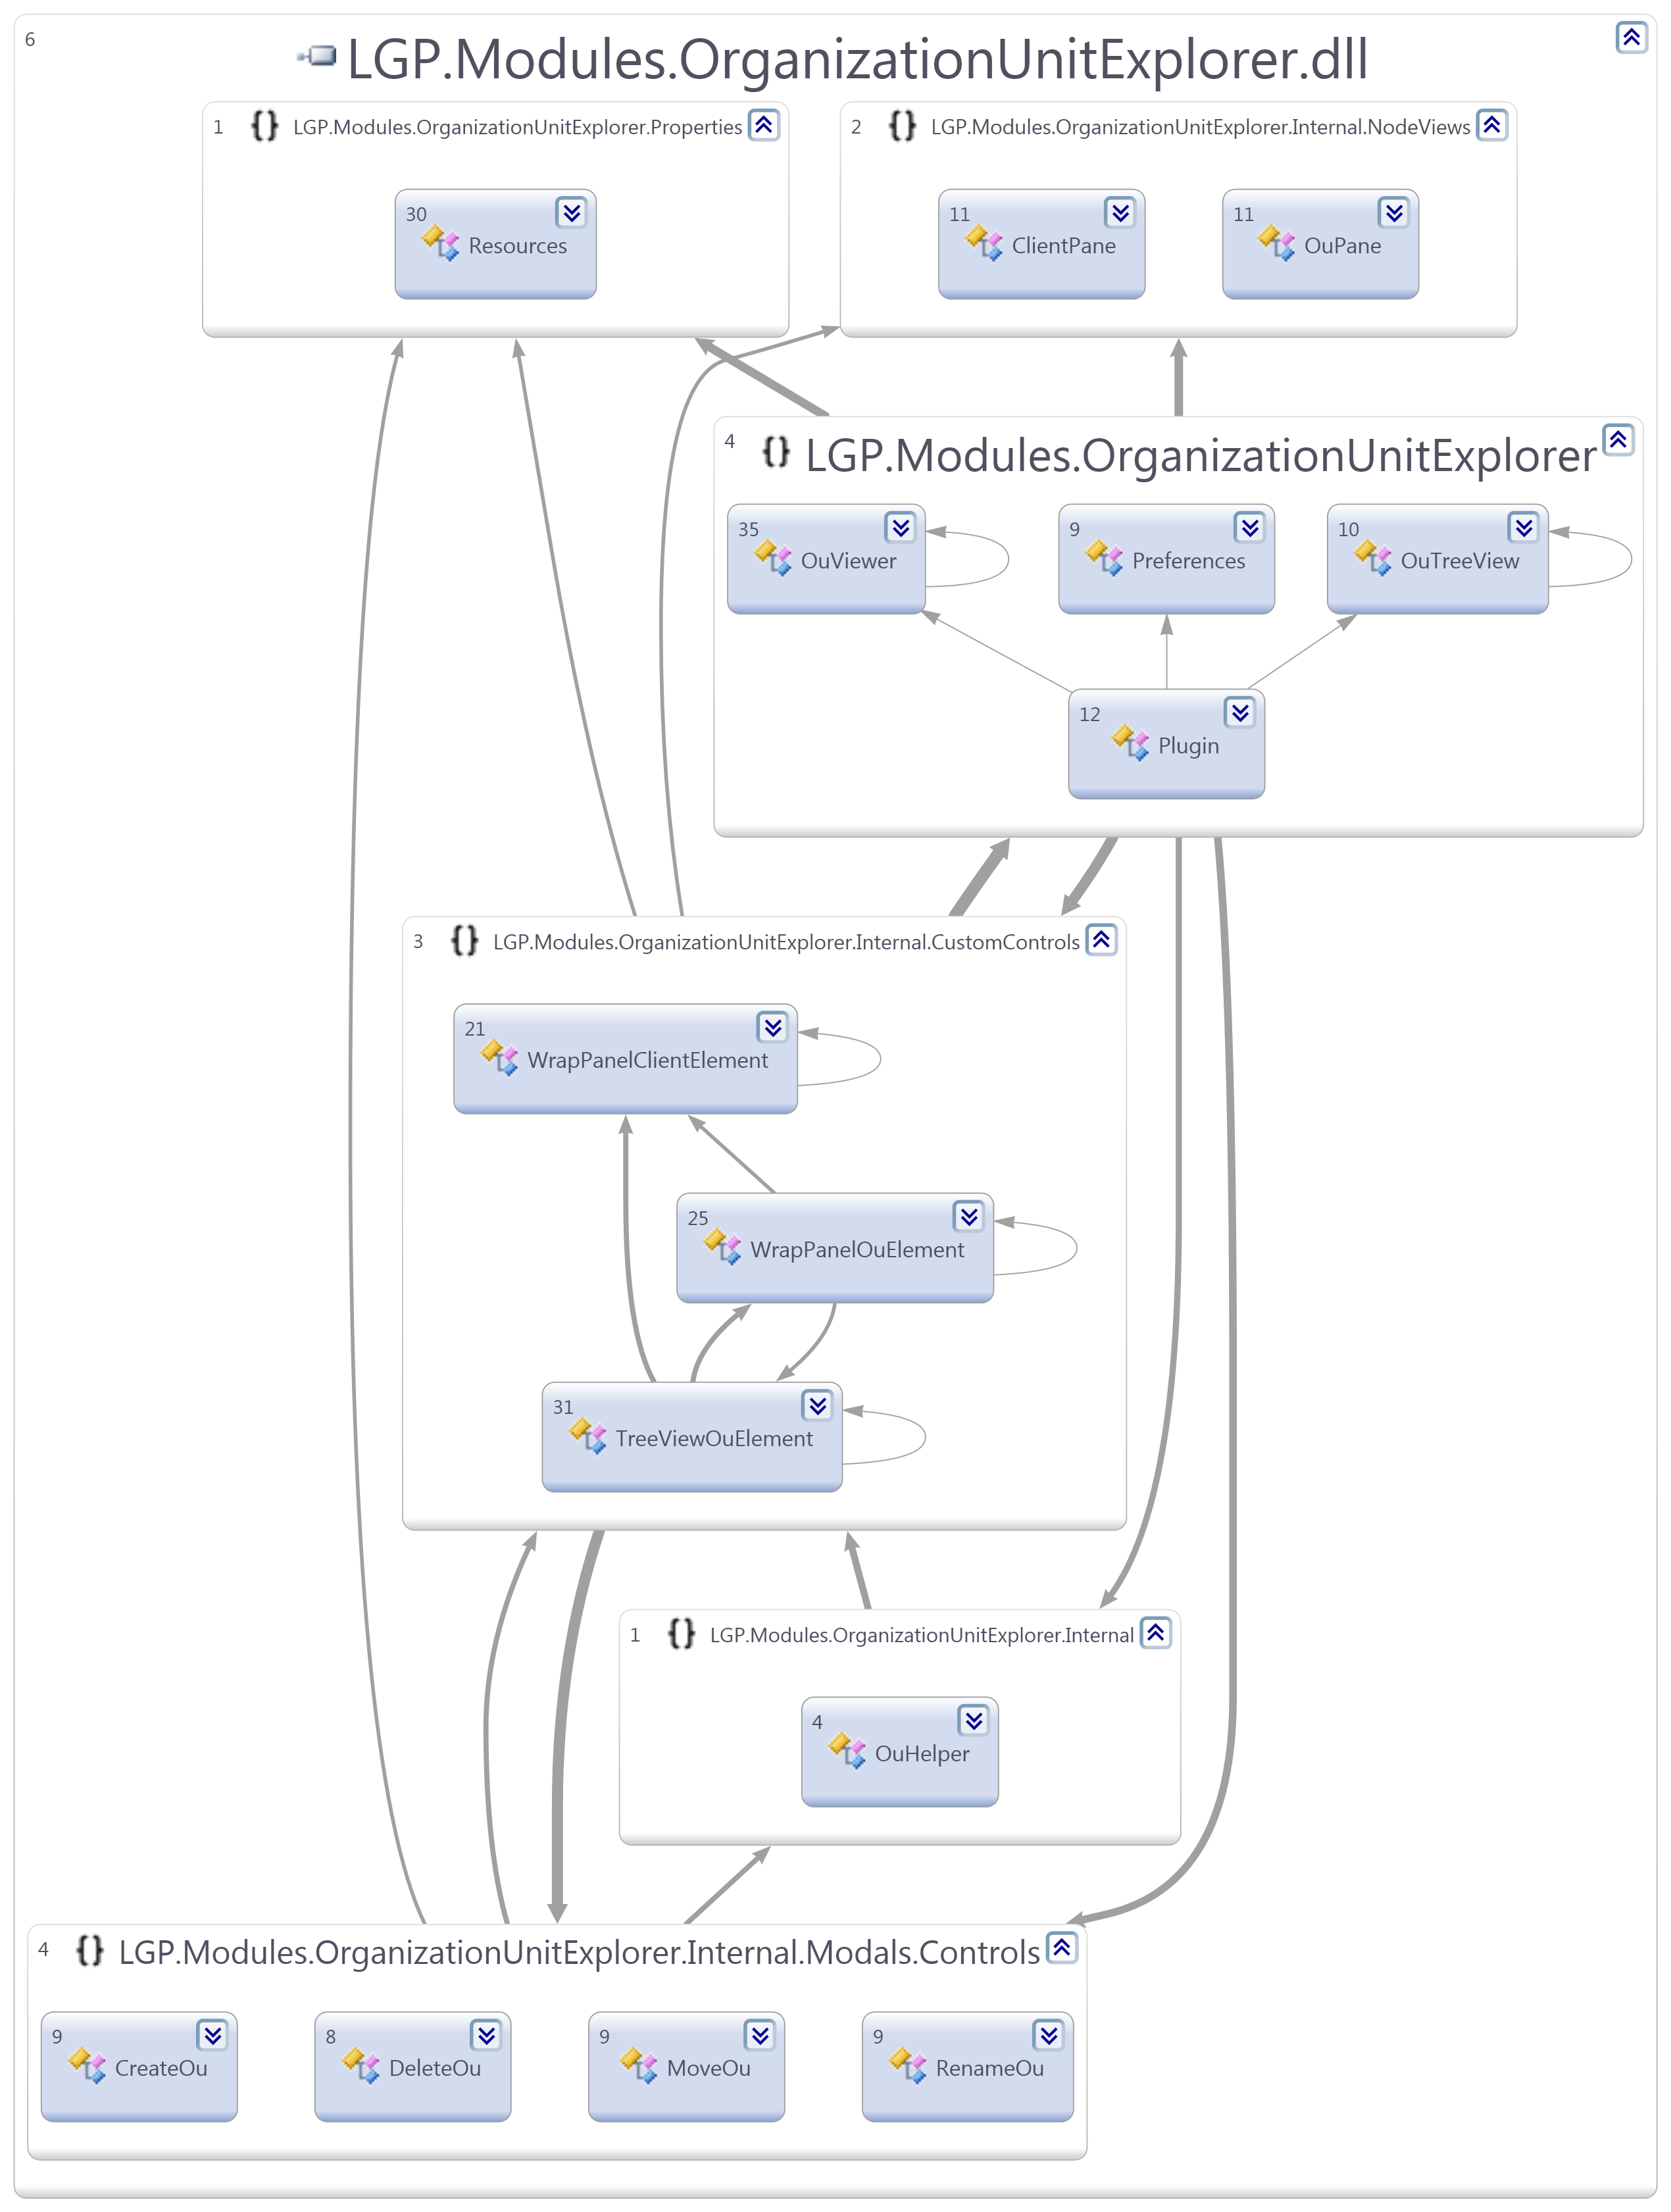
\includegraphics[scale=0.70]{pages/appendix3/figures/dllscreens/ou.png}
			\caption{LGP.Modules.OrganizationalUnitExplorer}
		\end{figurehere}
	

\newpage
	
	
	\large{\bfseries{LGP.Components.ModuleEditor}}
	\vspace{5mm}
	
		\begin{figurehere}
			\centering
			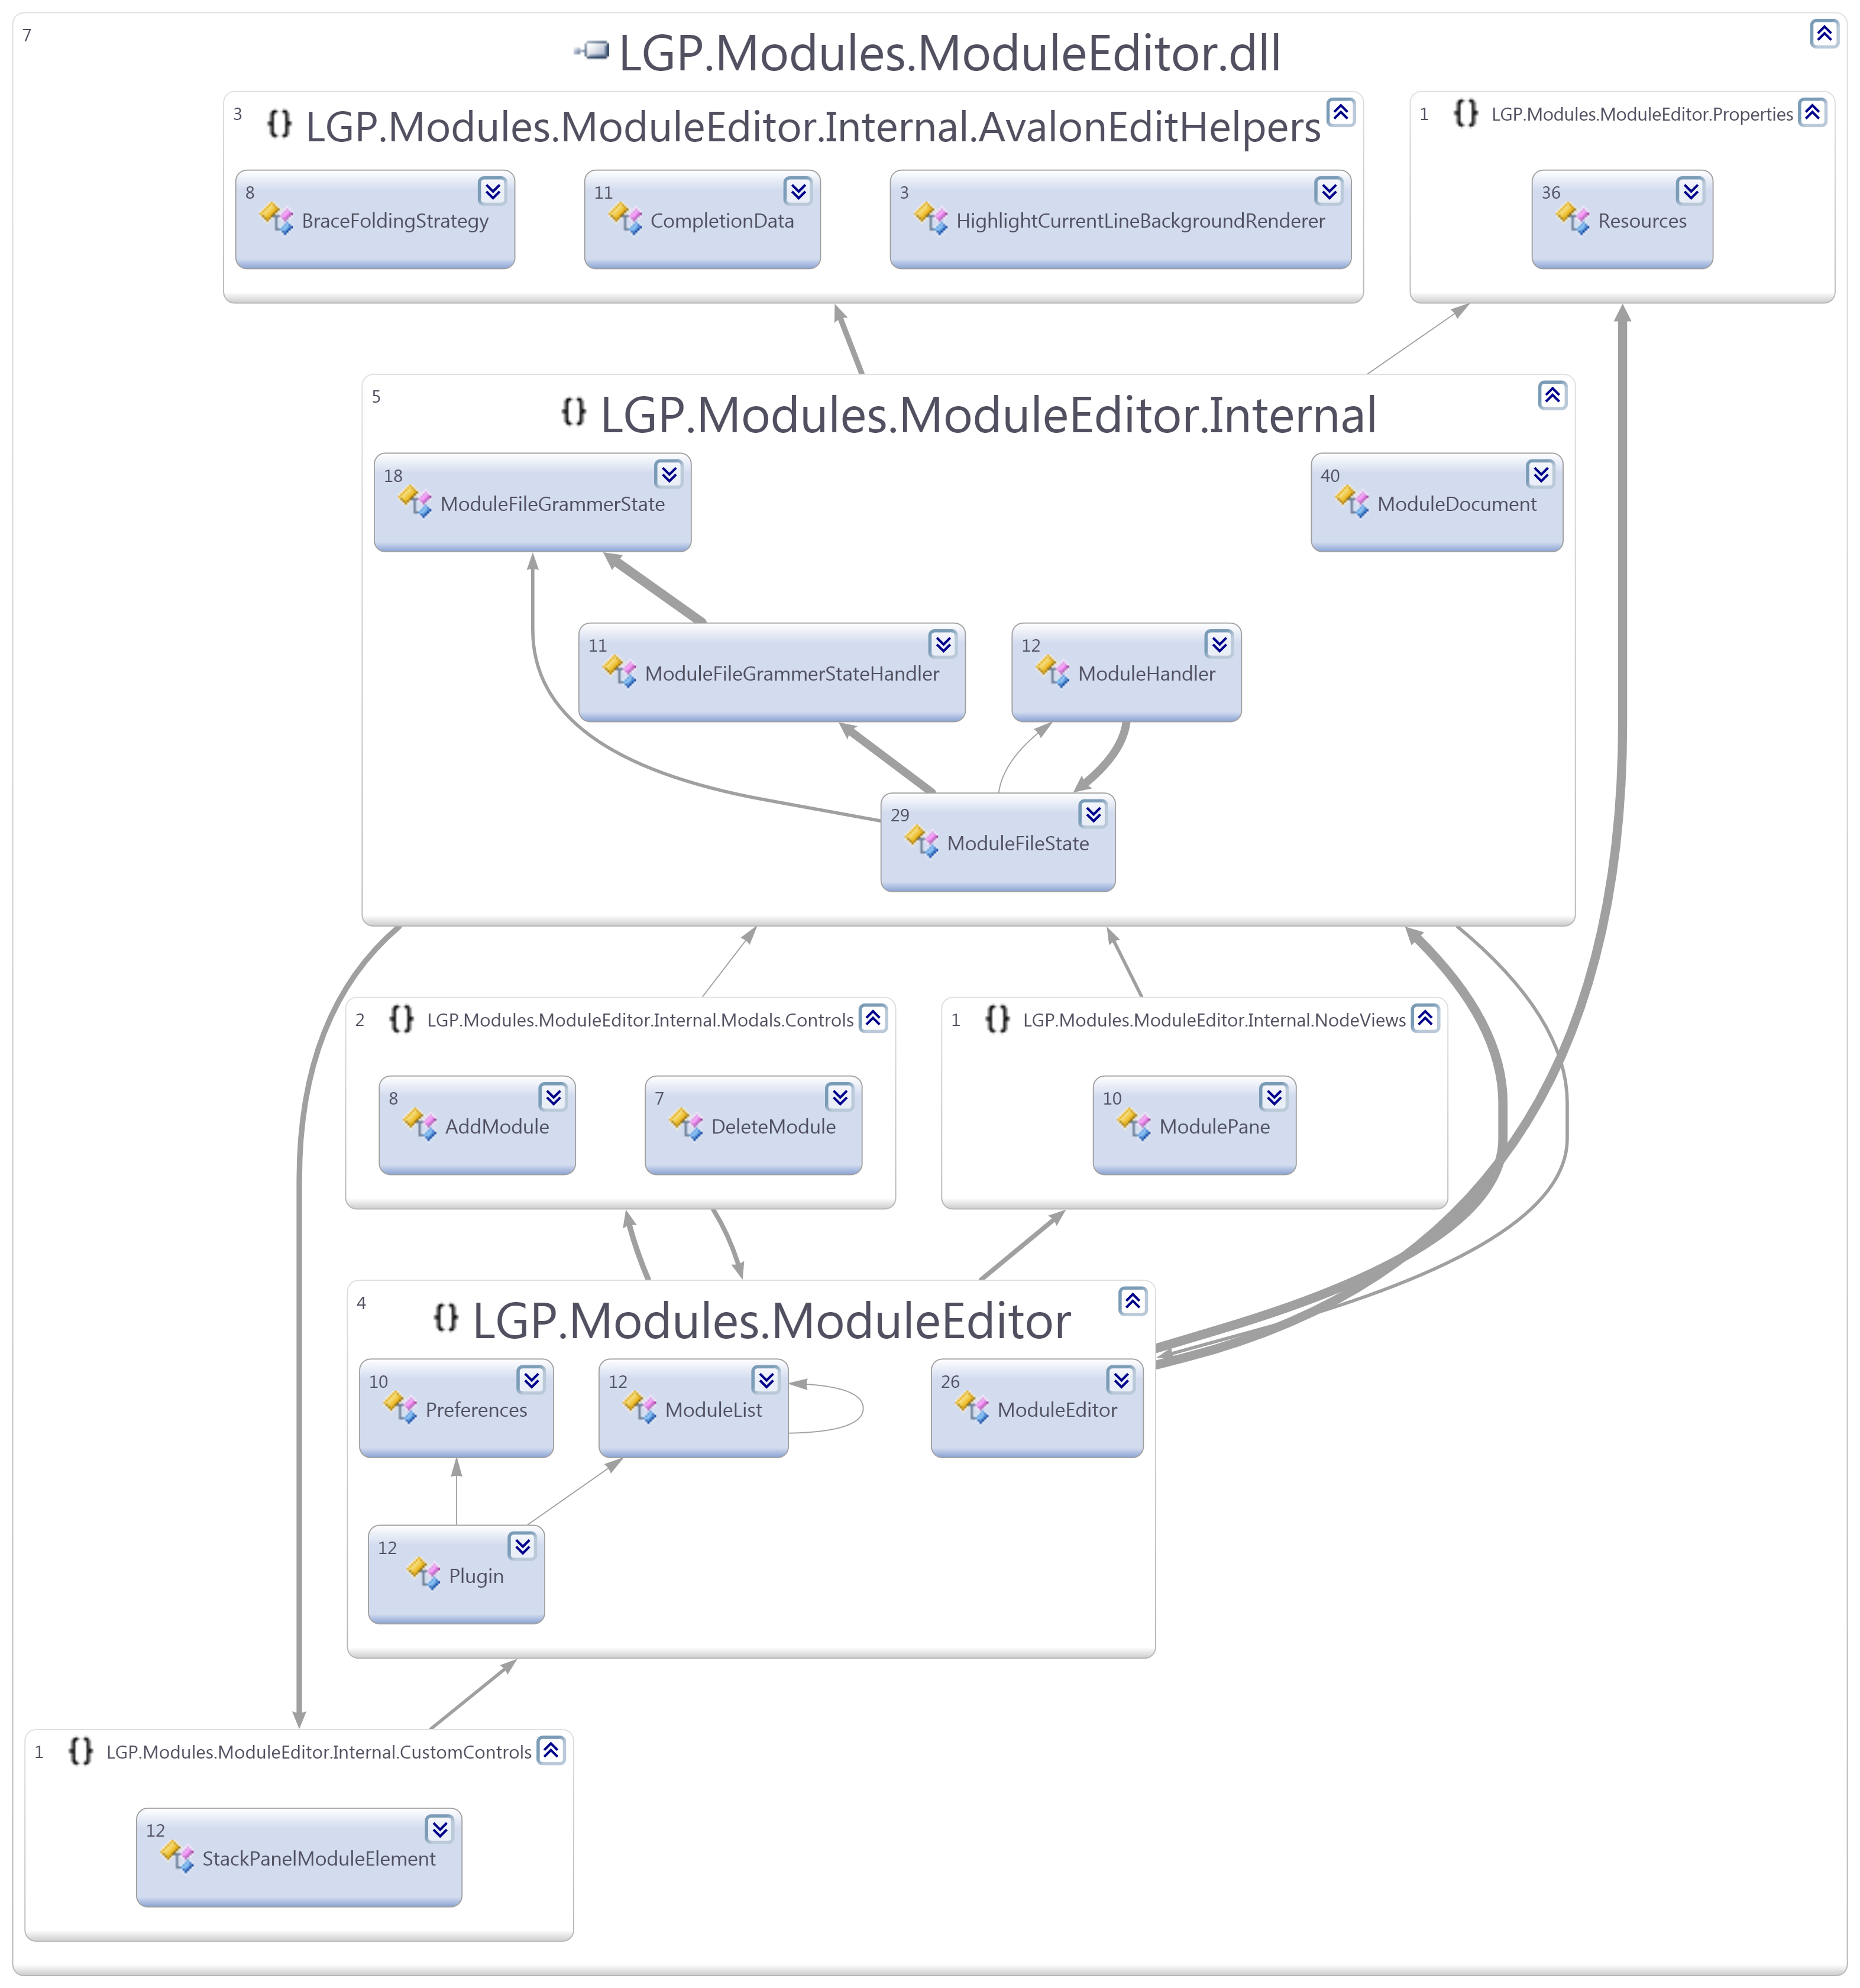
\includegraphics[scale=0.6]{pages/appendix3/figures/dllscreens/moduleeditor.png}
			\caption{LGP.Modules.ModuleEditor}
		\end{figurehere}
				
		
\newpage